

\documentclass[a4paper,12pt]{article}

\usepackage{xeCJK}
%\usepackage{ctex}

% 字体设置
\usepackage{amsmath}   % 数学符号
\usepackage{amssymb}   % 数学符号
\usepackage{amsfonts}  % 数学字体
\usepackage{graphicx}  % 插入图片
\usepackage{fancyhdr}  % 页眉页脚设置
\usepackage{geometry}  % 页面布局
\usepackage{hyperref}  % 超链接支持
\usepackage{listings}  % 程序代码显示
\usepackage{tikz}      % 绘图
\usetikzlibrary{matrix}% tikz矩阵库,必须导入
\usetikzlibrary{arrows.meta, positioning, calc} % 尖角箭头+位置调整
\usepackage{titlesec}  % 标题设置
\usepackage{fontspec}  % 字体支持(适用于XeLaTeX/LuaLaTeX)
\usepackage{setspace} %调行距的


% 页面布局
\geometry{left=2.5cm, right=2.5cm, top=3cm, bottom=3cm}

% 封面设置
\title{
    \vspace{-3cm}
    \Huge{\textbf{数字信号处理讲义}} \\
    \vspace{0.5cm}
    \Large{课程名称: 数字信号处理} \\
    \vspace{1.5cm}
    \Large{Digital Signal Processing} \\
    \vspace{2cm}
    \large{编写:刘健余} \\
    \vfill
    \Large{日期: \today}
}

\author{柳州职业技术大学} % 作者为空,封面不用显示作者
\date{}

% 页眉页脚设置
\pagestyle{fancy}
\fancyhf{}
\fancyhead[L]{数字信号处理讲义}
\fancyhead[C]{}
\fancyhead[R]{编写:刘健余}
\fancyfoot[C]{\thepage}

% 章节格式
\titleformat{\section}[block]{\normalfont\Large\bfseries}{\thesection}{1em}{}
\titleformat{\subsection}[runin]{\normalfont\large\bfseries}{\thesubsection}{1em}{}
\titleformat{\subsubsection}[runin]{\normalfont\normalsize\bfseries}{\thesubsubsection}{1em}{}


\setstretch{1.5}%行距1.5倍


\begin{document}

% 封面
\maketitle
\newpage

% 目录
\tableofcontents
\newpage

% 第一章
\section{Introduction}\quad

同学们好啊,我们开始上课。咱们这门课呢,是数字信号处理,那么在学习这门课之前呢,我希望大家有一些数学基础。但是不需要太多啊!只需要一些微积分的基础,要懂到什么程度呢?大概是会做一些基本的计算就行了。

\subsection{Digital vs Analog}\quad

那么我们来谈一谈咱们这门课,要学习些什么东西,也就是咱们整个学期应该要会的知识。我给大家列一个Sketch,数字和模拟。首先这个所谓“数字”,这是相对于“模拟”的概念。在之前的学习中,想必大家应当是学习过,比如电路、信号与系统,这样的课程的。那么信号与系统这门课的话呢,实际上与咱们这门课是有一些重合的知识点的,但是没关系,如果有基础好的同学,拿着一部分权当复习与听玩耍了。咱们这门课与信号与处理课重合的地方并不多啊,我希望的是给大家一些新的东西,新的知识点,至少是在描述上是直观的,但是在理论上也得严谨。



数字和模拟,他们是有一些比较的。一般来说,大家应当知道这些比较是怎么个事儿的,也就是说,我们为什么要研究数字方面的知识。因为,模拟的东西我们已经有所了解了,因为模拟电路大家应该有所接触,实际上我们在模拟这方面,能够做很多的事情的。那么数字,相对于模拟来说,它的优势在哪里呢?


咱们在这谈几个主要的点:


\begin{itemize}
    \item 1.\quad Programmable \quad Hardware $\Longrightarrow$   Software
\end{itemize}


第一个,数字的东西,是可编程的。这非常重要的啊!因为模拟的事情,它没法儿用编程来实现,只能够怎么样呢?只能够搭硬件!搭硬件这件事,它的灵活度,几乎就没有!你要想改变一点其中的东西,比如你想改变一点硬件的能力、一点性能参数或者一点任务指向,你就几乎只能重新搭。

这个所谓“可编程性”是从“硬件”到“软件”的转变,而软件给我们带来的灵活型是无以复加的。这是其一。

\begin{itemize}
    \item 2.\quad Accuracy \quad (Controllable)
\end{itemize}

其二,数字的精度非常高,它不但精度高,它还是个“可控”的精度。你比如,我们说可以用八位的精度来完成什么什么任务,要是位数不够,精度不够,我们可以搞12位,要是还不够,我们可以搞16位,甚至24位、32位。那你要说,不要那么高精度,你搞4位,也是可以的。这意味着什么?这意味着可以根据我的任务类型不同,根据我目标的差异,对我的精度进行控制。这是模拟干不来的,你说你怎么做到吧!你模拟的东西,怎么对精度进行定义,你要说多少多少位,那不好意思,你已经开始数字化了。你除了“多少多少位”之外,你还有对精度的描绘方法吗?好像没有噢!你只能面对示波器那个连续的曲线发呆,它显示多少,那就是多少,完全没有控制。

但是你要说,模拟的精度高,这个高低咱们且不论。呃,不知道在座的同学,有没有音响发烧友啊,就是那些听音乐的音响发烧友们,他们觉得最好的音乐都是模拟的,因为它一点量化误差都没有,所以最好的音响都是胆机。知道什么是胆机吗?没有任何数字器件,全是电子管,也就是说,所有的滤波放大都是用电子管做出来的,他们觉得那才是最原汁原味的音乐。光盘?是被他们鄙视的东西,因为这玩意是数字化的,一旦数字化,他就觉得你这个误差不可避免——你一数字那肯定就有误差了!那么他们都听什么玩意?他们都听黑胶,黑胶那个盘不是数字化的,那个盘基本上是一种模拟的存储。

好吧,那么精度这个事情,见仁见智了,咱们暂不与人争论。至少数字的,它的“可控性”,那是非常的好。那胆机基本上只有一个档次,那数字化的东西,那档次多了去了。

\begin{itemize}
    \item 3.\quad Storing \quad (Compression)
\end{itemize}

第三点,咱们讲这个存储。当然!数字的这个存储,可以把密度提得非常高,这一点是模拟比不了的。你看那个黑胶唱片,你看那个个头,比光盘要大多了,那MP3更别说了。它不但是存储密度很高,更重要的是,在存储的时候,你可以“压缩”,这一点模拟就完全没法比。因此,数字的优势。

\begin{itemize}
    \item 4.\quad Cost \quad 
\end{itemize}

再加一条!其实我们再加十条都是可以的,它的Cost是很低的。啊咱们都是电子信息专业的啊,或者是学计算机的,咱们对咱们这个行当,应该有一些直观的理解与认知的——就是说Cost这个东西,大家知道应该怎么样才能低吗?

就一句话,任何一种产品,你如果能把它做到硅(Silicon)上去,那么这个Cost就不需要考虑;反过来说,你不能把它做到硅上去,那你的Cost Down就基本上是一句空话。硅,基本上可以理解为沙子,没啥区别,二氧化硅就是沙子。芯片的价值,百分之九十九点九九,很多个九,都是附加价值,什么意思,你一块芯片,邦,掰成两半,不值钱了;但是你一块金子,你掰两半,绝对一半还有一半的价值——差别在哪?本质上那个芯片的原料,本质上就是二氧化硅,他就是沙子,取之不尽,用之不竭,所有的价值都是附加上去的,这才叫高科技。为什么说信息产业是高科技?其实核心的点,就在于我们是在用智慧附加值取代传统的材料价值。因此,对数字端来说,它的Cost一定很低,因为它可以做到硅上去。当然,模拟的也不是说做不上去,现在模拟集成电路也挺流行的,但是难度大多了。模拟集成电路的设计,包括模拟集成电路工程师的培养、包括他的学习曲线都和数字集成电路不在一个层面上。


好,所以大家看,数字相对于模拟而言,优势很大。我们学习数字信号处理,其原因就在于此。我们想把握住时代的脉搏,或者说跟上时代的脚步,不至于被落下,我们就得对数字有深刻的体会和理解。


\subsection{Preliminary for Digital}\quad

咱们这门课将会从七个方面逐次展开。那么,第一个方面——\textbf{信号与系统}。


信号与系统大家应该都学过了,但是呢,大家学习的重点应该是模拟的,或者说是连续的,离散的应该也学过,所以说咱们的课程内容会有部分重叠。那么,我希望能帮助大家做一点复习,帮大家回忆回忆,课程与课程之间稍微有一点重叠,这是课程体系必须的啊。

那么我们这一部分的话呢,主要从\textbf{时域}和\textbf{频域}这两个域展开。


第二个方面——怎样得到\textbf{数字信号}。

我们要想处理数字信号,那么首先得得到数字信号是吧,这毫无疑问!我们要想得到数字信号的话,就一定是需要所谓\textbf{A/D}技术,也就是\textbf{采样}(Sampling)。这是我们信号处理的前提,也是我们信号处理的基础。我们有了采样技术,才能完成从现实世界到数字世界的转变。


现实世界都是连续的,没有离散的东西。数字世界在我们建构在我们头脑当中的,所以说,什么叫虚拟,什么叫现实。从咱们这门课开始,我们就在接触这样的哲学概念。数字的都是虚拟的。

那么现在有一个更加吸引人也更加流行的词,叫数字孪生(Digtal Twin)。就是说,我要在我的数字世界里面,完成对于现实世界的完美呈现。我要让数字世界中产生一个跟现实世界我所思考的对象完全相同的对象,只不过两者之间,一个是现实中的,一个是我们头脑当中的,或者应当说,是计算机的头脑当中的。两者的运行规律,两者的特点呈现是完全一样的。这几年很流行!我们这门课就是在做这玩意,尽管说,我们不像真正的数字孪生搞得那么复杂,但是从哲学上来讲,我们完成了AD采样后,就是在做这件事情。我们的AD采样是要尽可能地去复现出,我们原有的现实世界的一切的。


当然了,除了A/D之外,还有所谓的\textbf{D/A},因为我们不可能总在虚拟世界中。我们终归要回到现实世界,才能够帮助我们改造它。所以,D/A和A/D相辅相成,这是我们如何得到数字信号。


然后,我们就得考虑一下,怎么去\textbf{处理数字信号}(Process Digital Signal)。这应该是第三点了啊!

那么,我们怎么处理数字信号呢,这是我们学习的核心内容。这里我们将从两个层面来展开,这个事情的话呢,是我们得先有一些基本工具:一个是\textbf{傅里叶变换}(Fourier Transform)和一个是\textbf{Z变换}(Z-Transform)。这是我们的基本工具。那么除了基本工具之外,我们要给大家介绍我们处理数字信号的一个基本的方法,所谓\textbf{线性滤波}(Linear Filtering)。


也就是说,我们希望能够把滤波操作,作为数字信号处理的核心介绍给大家。当然了,这个线性滤波也有很丰富的内容。你比如,有滤波器的表示方法(Representation),其中最核心的就是\textbf{卷积}(Discrete Convolution),当然了,是离散卷积。因为卷积这件事情,大家其实并不陌生,在信号与系统中大家都学过。


那么,我们还有滤波器的实现(Implementation),实现强调的是时域和频域之间相互的映照。咱们数字信号处理工程师,脑子里时时刻刻都是双轨制,怎么个双轨制?时域和频域,两个轨道,两种路线,两个视角,时时刻刻,同时出现,这才是一个工程师思维。


然后的话呢,我们还得谈一点架构(Architecture)。我们为什么要谈一些架构呢?是因为我们做信号处理,一方面是为了得到处理的结果,另一方面我们是希望把方法固化。换句话说,我们希望从软件进展到芯片。架构,这是芯片思维,我们从架构上是能够,呃,尽管还没有走到啊——但是是能够去感受到芯片带给我们的那种激动。好的!这是我们的线性滤波。


好!第四个方面!然后我们会谈到什么呢,谈到怎么样能够改善我们的\textbf{处理性能}(Improve Performance)。


我们仅仅知道要怎么做,这是不够的,我们还要知道怎么做能做得更好!怎么叫做得更好呢?这里我们将强调两个方面——当然,性能这个东西要涉及的内容那是相当的多了——我们强调两个方面:第一个方面,我们希望做得更快。因此我们将要给大家介绍最伟大的算法之一,所谓\textbf{快速傅里叶变换}(FFT)。快速傅里叶变换是20世纪十大算法之一,说它是最伟大的算法之一毫不过分!这个基本上,业界上,有一说一,大家没能否认!就在咱们这门课上,我们就要接触到它了。这是怎么样能做得更快。


第二个事情是,怎么样能做得更准。这里有两个层面的事,一个层面是所谓\textbf{量化噪声}(Quantization Noise)。这就是刚才我们所说过的,那些顶级的发烧友们去诟病数字的地方。他们觉得,你数字的东西,你不可能是无限精度的!任何一件事情,只要进了计算机,它的精度就受限于你计算机的处理字长(Word Length),所以这里你不可能去回避你的量化噪声。当然,与之相关联的,所谓的\textbf{有限字长效应}(Finite Word Length Effect)。这是提高精度的关键,我们要了解这其中的一些基本概念。当然,在我们这门课上,我们没有办法去完全地展开介绍如何提高精度所需要的技术,但是我们希望在一两节课之内,让大家对这个基本概念有所认识,让大家知道我们在这里面临的是什么样的问题,处理这样的问题,它的难度在哪里,我们基本的处理思路是什么。具体的技术,我们不一定能够有效地展开。


好的,然后我们会谈到第五件事,我们如何来具体地\textbf{设计滤波器}(Design Linear Filter)。强调一下啊,我们的滤波器设计,和我们关于滤波器内部工作机理的阐述,这是两件事。在工程领域,包括我们各门课程,大家对于课程内容需要有一个自己的比较鉴别分类。不同的内容,它的指向是不一样的。设计这意味着什么?设计这意味着,一定是任务驱动(Task Driven)。就是我要有具体的任务,我怎么样来通过对滤波器架构的选择,怎么样通过对滤波器参数的优化,来达成我所预定的任务,这叫设计滤波器。之前咱们说的那些什么变换什么的,那都是和任务没关系的,那都是滤波器内部的工作机理。而任务,是有外在接口的。因此,设计滤波器,这是专门的内容。


那么,我们在设计滤波器当中呢,重点谈两种架构的滤波器。一种叫做\textbf{有限冲激响应}(Finite Impulse Response,FIR)。一种叫做\textbf{无限冲激响应}(Infinite Impulse Response,IIR)。我们重点谈这么两种,这也是咱们信号处理的经典内容。我们需要强调,在这一部分呢,我们给大家更多的是,谈论的是一些基本的设计思路,一些idea。因为具体的实现部分,应当是日新月异的。现在在我们数字设计的领域,工具的迭代速度是远远超过人们的想象的。基本上咱们在大学期间熟悉了某种设计工具,到你毕业的时候就过时了。基本是这么一回事啊,所以呢,咱们的学习,切记不要舍本逐末,不需要去追求那些工具的使用与熟练。因为你用得再熟,它的过时也是不可避免的。因此我们更需要把这个idea看得清楚,因为这才是我们未来有可能去创新的根本——你的工具掌握得再熟练,也跟创新没有一毛钱关系。


那么我们,应该还得介绍一件事,应当是所谓\textbf{希尔伯特变换}。这是一种特殊的滤波器,但是它在我们数字信号处理的世界里面,占据着一个非常重要的地位。


好的!我们,现在已经对数字滤波器有了从机理到设计的全方位认知。我们还需要对它进行扩展,这应该是,第六件事!对\textbf{线性滤波器的扩展}(Extend Linear Filters)。

我们的扩展呢,主要也是两个方面:一个方面,我们希望能够从\textbf{实信号}(Real Signal)扩展到\textbf{复信号}(Complex Signal)。我们会跟大家来解释这件事情,因为复信号这东西又有点形而上了。这个东西是虚拟的,现实生活中哪有复数啊?但是我们确实需要这个虚拟的架构,其原因在于,如果我们没有复信号的概念,我们甚至建立不起来对于一些非常基础的概念的准确认知。比方说相位,没有复数我们甚至没法准确说出来什么是相位,但是有了复数就不一样了,而大量的信息是在相位里的。你想想看,通信把信息调制在相位上,这是基本的操作;雷达回波的信息,几乎全在相位里——距离、速度、角度全在相位里;导航,声呐,无疑不是对相位非常重视的。因此,复信号,几乎是必须的。

然后我们还会谈,所谓Multirate,这叫\textbf{多速率}。多速率这件事,在现代数字信号处理乃至于现代信息处理里面都非常常见。它为什么很重要,给大家简单的解释一下。就是说,我们无论是做信号处理也好,还是做信息处理也罢,我们时时刻刻都要面临一个问题——就是我处理的细致程度到什么一个点就可以了。因为你这个处理啊,你细致,这件事是永无止境的,就好像一幅图,什么分辨率,20$\times$20,这也不是说什么也不能做啊!这个著名的MNIST手写数据集就是28$\times$28的小小的图,它处理一个手写数字,足够了。但是如果你想来点风景,来点人脸,来点稍微上台面的东西,你就得几百乘几百。可是几百乘几百呢,你很多信息实际上是看不见的!比方说,国家电网用无人机,做高压线的巡线,它是要准确地拍到那个高压线的那根线的,你可以去尝试一下啊,如果说它仅仅是几百乘几百的分辨率,你那个照片拿出来那根线啊,忽有忽没有的,你根本就看不清楚!所以,几百乘几百肯定是不行的。4k乘4k?OK,那这个线看着是非常清晰了,这就没问题了!可是,你如果是4k乘4k这样的分辨率,对于它某些应用场合去辨别特征目标的细部特征,那就不是很够用了!那你说我8k乘8k!16k乘16k!这个东西永无止境!核心在哪?核心就在于,你要对于这个任务啊,要有所认知。什么样的任务,什么样的目标,决定于你能做到什么样的程度。可是,我们获取的数据往往不能够随任务随心所欲地改变,刚才我们说数据都是老天爷给的,你不能要求老天爷什么。老天爷给你什么样的东西,你就只能在什么样的东西上工作,这个东西你改变不了。因此,万一要是数据它的分辨率也好,它的细微程度也罢,与你的任务不匹配,那你咋整?你只能,借助于Multirate技术,你要对它进行适当地升采样以及降采样,你才可以根据你的任务对你的数据进行合理地适配,以至于让你可以很好地去完成任务。因此,我们要给大家介绍Multirate技术。


最后一部分,第七部分,怎么样去\textbf{应用线性滤波器}(Apply Linear Filters)。我们前面说的天花乱坠啊,我们这个滤波器的内部工作机理,我们这个滤波器的外部设计接口,我们滤波器的各种各样的扩展形式,全部都还是浮在空中的,没有落到地面上来。要落到地面上来,我们一定得把它用到我们实际的数字系统当中去。因此,我们要告诉大家的是什么?大家千万不要觉得说,啊我只是一个普通的大学生,我只是在学习一门本科的非常基础的课程,我并没有学到什么多么高深的知识,并没有学到多么花哨的技术,因此我做不了什么事情——千万不要这么觉得!我们在这想告诉大家的是什么呢?我们的统信,我们的雷达,这里的雷达包括我们的脉冲雷达(Pulse),包括我们的调频连续波(FWCW),包括我们的SAR,还有我们的计算机断层造影(CT),我们的核磁共振(MRI)。所有这些东西,说到底,就是一个FFT,你相信吗?通信当然我们说得宽泛了点,我们就说5G吧!5G的最底层的逻辑叫OFDM,OFDM说到底它也是一个FFT。就是你用FFT就可以把它基础的处理完成,所以某种意义上讲,我们这门课学完了,你就可以找工作了,如果你能把这门课的知识都掌握到位的话,你就真的可以去找工作了。

好的,这就是我们这一门课的一个知识梗概。我希望大家能对我们学习的内容有提前的了解啊,这样我们回去呢也可以把我们这个内容的Sketch与那本奥本海姆的教科书啊,做一下对应。因为我们应当是大概地把那一本教科书的内容覆盖了差不多70$\%$。其中有一部分内容,我们没有刻意想去覆盖的原因是因为它可能需要的先验知识有一点点多,比方说随机信号。


\subsection{History}\quad

好,剩下的这点时间的话呢,我想给大家稍微谈论一点我们这门学科的历史,我指的是数字信号处理的历史。了解一点历史对于激发大家的学习兴趣,还是有一定作用的啊!

我们这门学科的历史其实很长,大概1730年的时候就有了,因为这个时候傅里叶(Fourier)就出现了。傅里叶在1730年的时候啊,写了一本书,这本书原本是关于什么的呢?是关于热传播(Heat Transfer)的,啊当然了,这事跟咱们这个学习不是特别的有关系。但是,他推出了一套工具,叫做傅里叶变换。这个工具太重要了!傅里叶变换是人类历史上影响力最大的一种分析工具,它直接指向简谐运动。它认为任何一种复杂运动都可以分解为简谐振动的线性叠加——这个思想太光辉了!这使得我们面对任何的复杂都不再惧怕,因为我们知道,只要把它分解成若干个简单的研究对象,我们就有把握把它研究清楚。而这个简单的研究对象就是简谐运动,说得更准确一点,就是我们的\text{sin}和\text{cos},也可以写成$e^{j\omega t}$,这是傅里叶的洞见。其实后人考古啊,发现这其实不是傅里叶创建的,就是他前面还有很多先哲有更加原创的想法。傅里叶他其实是一个总结者而不是一个创新者,不过由此也可以让大家看到,会总结也是很重要的——谁知道后人会怎么看这个事情?也许后人看到的就是这是你写的一份很好的总结,然后就把所有的功劳都归到你头上了,这个也难说。


好啊,那么再往下,好长时间很沉寂。电学的历史啊,很近。下一个大概是1900年,是马可尼(Marconi),马可尼发现了一件什么事?马可尼发现电磁波就是简谐振动,他的这个发现,使得傅里叶他关于热的这些个理论方法立马很自然地传达到电身上。因此,奠定了傅里叶变换是我们研究问题的基本工具的这么一个局面。


然后再往下大概是1930年,1930年呢,有一群人在研究控制问题。有个人叫Bode,他或者说当时有这么一群人,他们在研究控制理论(Control)。但是在控制的时候,他们已经提出了关于信号处理(Signal Processing)的一些基本问题了。控制和信号处理,本质上是一回事,为什么呢?是因为,什么是控制?我首先要感知情况,其次是要改变情况,两部曲。我怎么感知情况?我通过采样数据,实现对目前情况的认知。我要从采样数据当中提取出关于目前情况的有效信息,你说这不是信号处理是什么?所以信号处理是控制的第一步。当然第二步是,它要用控制手段来对目前情况的运转状态进行有效地变化,因为要希望它运转向自己期待的那个方向与角度,当然这是另外一个问题。但信号处理这一定是前提。在1930年代,人们就已经有所认知了。


然后我们,到1940年代,40年代发生了两件事。这两件事的核心其实是一件事,因为这时候爆发了第二次世界大战。第二次世界大战对于信号处理的推动是决定性的,以至于我们直到今天为止,我们信号处理的核心结果,它的基础都是第二次世界大战当中奠定的。


当时有两拨人在工作,这个当然大家都知道啊,一拨是美国人,一拨是苏联人。那么美国人呢,他的典型的代表是维纳(Wiener)——著名的维纳滤波就是在当时提出来的。然后苏联人的典型代表是Kolmogorov,那么Kolmogorov实际上是从更加一般化的角度,从更加理论的角度,对维纳滤波进行了很好地阐释。所以,他们当时所奠定的是\textbf{最优滤波}(Optimal Filtering)的基础。这个基础,直到今天仍然是数字信号处理的核心内容。可是很可惜!我们这门课覆盖不到!为什么呢?因为它需要一个前序的课程,这个课程叫随机过程。我知道大家应当都学过概率论,暂且不论大家学的水平如何,但是呢,随机过程我估计大家应该是没有学过的。就是,它需要随机过程作为一个前序基础,我们才能够更好地理解这个最优滤波。所以,尽管从时间顺序,它出现得更早,但可惜我们这门课它没法覆盖。那么这一个内容,或许会在将来咱们研究生一年级的现代数字信号处理那个课里面来讲授。就是我们研究生一年级,将会对数字信号处理的课程有一个延伸。在现代数字信号处理中,我们将利用统计工具帮助大家扫清障碍,然后来认识维纳滤波。这是一个方面。


第二个方面,在40年代发生了一件对于信号处理非常关键的事情。就是有一个叫奈奎斯特(Nyquist)的人,他给出了采样定理,更准确地讲应该叫奈奎斯特-香农采样定理(Nyquist-Shannon Sampling Theorem)——香农是信息论之父啊,通信领域的祖师爷,这个大家都知道啊——那么采样定理,从理论上,完成了我们对于模拟到数字,连续到离散的一个基本认知。所以采样定理,这个在我们的课程之中是要覆盖的。这是刚才我们所说的第二个内容。好的,这是40年代。



然后到50年代,信号处理又有了突飞猛进地发展。这个发展主要是依赖于什么呢,主要是依赖于航空航天——更准确地讲,是阿波罗计划(Apollo)。就是当时美苏冷战,使得双方把大量的资源投入到航空航天领域,以至于相关的技术飞速发展。具体到我们信号处理当中,产生了一个技术叫卡尔曼滤波(Kalman Filtering)。非常可惜,这个卡尔曼滤波在咱们的课程里也覆盖不了!是因为它也需要一些先验知识,主要也是从随机过程当中来的先验知识。这个也是在我们研究生的课程当中,将会对卡尔曼滤波进行比较详细地介绍。


随后,时间就来到了60年代。60年代,是被认为我们数字信号处理,真正意义上的数字信号处理的缘起之年。1965年,FFT技术横空出世,这主要是两个人,一个叫Cooley,一个叫Tukey,贝尔实验室的人。FFT技术的出现,很多学者都认为是信号处理真正意义上的开始。因为在FFT技术出现之前啊,我们的数字信号处理处在一个不尴不尬的境地,为什么呢?从理论上讲,信号处理的基础理论,实际上已经把我们远远地甩在后面了——从三四十年代开始,大量非常优秀的数学家和物理学家投入到信号处理领域,由于第二次世界大战的激励,由于阿波罗计划的激励,使得他们在理论上的积淀,事实上是做得非常超前的——按今天的观点看来都一点不落后。但是啊,你数字信号处理和前人比理论你是比不了的,而你要想落地呢,你又落不下去。它为什么落不下去,是因为计算复杂度使得当年的计算设备完全没有办法去承担你的这种处理任务。这样一来,你这个学科就变得高不成低不就——你要想够理论呢,人家理论又远远超过你;你要想落地应用呢,你又落不下去——不尴不尬。这种局面的终结就是FFT!FFT一来,使得一下子这个信号处理就可以到处用,确实就可以到处使用了。我们刚才说,所有这些其实就是一个FFT。因此,信号处理就真正地开始了。这件事情,我们的课程是肯定要覆盖的。


然后呢,时间就到了1980年代。这个时候,有一个东西出现了,这个东西也叫DSP。哎!大家不要把它跟我们的信号处理混为一谈啊!这个东西是Processor,不是Processing,它是一种CPU,一种特殊的CPU,专门用来干信号处理的CPU。这个CPU和普通的CPU相比较,两大特点——当然今天其实两者在融合啊,今天整个的计算架构已经和当年完全不一样了,但是按当年的说法——两大特点:第一个特点,它这个CPU的效率,执行效率要比普通的CPU高——做信号处理相关计算。我举个例子,它一乘一加可以在一拍之内做出来,就是一个时钟周期可以做一乘一加两个动作。你想想看,我们信号处理,我就随便写一个公式啊,就随便写一个,你比如说
\begin{equation}
    \sum_{k=1}^n \alpha_k X(k) 
\end{equation}
这个东西不就是信号处理常干的事吗,这不就是个典型的线性滤波吗?那么你如果把它拆开看,它是不是乘一下,加一下,乘一下,加一下,没错吧!一乘一加,DSP可以在一拍之内给它完成,所以它干这种活特别有效率,此其一。其二呢,它功耗低,相比于普通CPU功耗低。因此更适合部署到前端去,而不是云端,按今天的说法叫部署到边缘端——要更靠近现场,更靠近我们处理的对象。出现了Processor,这使得我们信号处理一下子成为了信息社会的主流技术。包括我们的Speech、Audio、Image、Video,你就想像吧,我们的生活真的是被信号处理改变了。就在现在这个时刻,你手里持有的信息化的各种各样的设备,无一例外,全部装备有DSP,无一例外,大小而已——可能有的大,有的小,有的是作为SOC的一部分,有的是Stand alone的,是单独的——但是全部都装有DSP这个东西。我们每时每刻都在享受着信号处理给我们带来的好处,它真的是改变了这个世界的样子。所以说,我们没有理由去拒绝它的诱惑,我们没有理由去不学习这样一种真正能够让我们体会到能改变世界的这种快乐的技术,这就是我们的数字信号处理。OK,我们今天就先到这,我们今天没有什么实际内容。从下节课开始,我们正式地进入到数字信号处理的学习。好,我们就到这吧。

\newpage
\section{Discrete Signal and Discrete System \uppercase\expandafter{\romannumeral 1}}\quad

好,我们开始上课啊。今天开始,我们要正式学习数字信号处理。那么我们首先要给大家做一些概念上的铺垫,主要是离散信号与系统。信号与系统大家都已经学过了,不过呢,在信号与系统课程当中,学习的重点应该是连续的信号与系统。离散部分呢,我相信可能也有一些提及,但是可能并没有学习得非常地系统和深入。所以,今天我们先要对这一部分知识啊,进行一下铺垫。如果大家对这一部分知识掌握得已经很好了,那么大家就当是复习;如果大家不是很熟悉的话,那么今天的学习对于今后的学习而言,还是非常的重要的。

\subsection{Discrete Signal}\quad

我们说一个信号$X(t)$,信号是什么东西?它有两个要素:第一个要素,它有一个自变量。这个自变量啊,有的时候我们可以认为它是时间;有的时候呢,我们可以认为它是空间,所以它未必有明确的物理含义,这并不是很重要。第二个要素,一个信号,它有自变量,有因变量,因此,它本质上就是一个函数(Function)。我们对于函数啊,非常的熟悉。因为我们从中学开始,就会知道这个函数嘛,它通常会有一些解析的表达,你比如$t^2$、$3t^3$之类。而现在我们所研究的信号呢,通常具有什么样的特点呢,就是它并没有明确的解析表达式。解析表达这件事,书本上见得比较多,现实当中非常的少,所以这明显是纸上谈兵的一个产物。我们在现实当中所遇到的信号,它的解析表达我们往往是不清楚的,因此我们才要对它进行处理。那你想想看,如果它的解析表达我们都已经非常明白了,我要处理它干什么呢,我们就直接应用它就好了。我们处理,就是为了能够从信号的值当中去获取信息,帮助我们对这个信号深入地进行认知。


离散的信号,什么意思呢?我们要进行采样的
\begin{equation}
    X(nT)\quad n\in \mathbb{N}\quad T\in \mathbb{R}
\end{equation}
这里的$n$是一个整数,而这个$T$呢,往往是一个实数。我们要进行采样,采样的意思就是说,我并不是对连续数轴上的每一个自变量都能够获得信号的值,我只能获得它在一些离散的时间点上的值。

我们为什么对于采样这件事很感兴趣,我们上一堂课已经说过了——如果它是连续的,其实我们处理起来并不是很容易,而且呢,我们处理之后所获得的收益也并不一定很大。数字信号相对于模拟信号而言,优势非常明显,因此我们进行采样。而一旦进行采样,这个信号的形式啊,它就发生了比较明显的变化——它的自变量就变成离散的了。为了可以比较明确啊,很多的文献会这么写$X_a(nT)$,在这里加一个$a$,加一个$a$这个说法比较讲究——这说明这个信号原本是一个连续信号,而我们在离散的点上对它进行采样,那么我们可以进一步把它记作
\begin{equation}
    X_a(nT)\quad \Longrightarrow \quad x(n)
\end{equation}
所以这就是我们信号处理的研究对象。

我们在这啊,要提出两个比较典型的离散信号。第一个是所谓的$\delta$
\begin{equation}
\delta(n) = 
\left\{\begin{matrix} 
  1\quad n=0 \\  
  0\quad n\neq 0 
\end{matrix}\right. 
\end{equation}
$\delta$这个东西大家都很熟悉啊,所谓的“冲激”(Impulse)。冲激可以帮助我们干什么事呢?它可以帮助我们做这么一件事:我们看任何一个离散信号,我都可以把它用冲激来进行表达。这样的表达在我们信号处理当中,是一个永恒的话题。怎么讲?我们希望能够用相对比较简单的对象,来表达复杂对象。我们希望这种表达是一种分解,这个分解的结果应该是一个线性叠加。这样的一种思想,我们今后要反复使用——对于一个复杂信号,我们总希望用简单信号的线性叠加对它进行表达。我们很快就会知道这个表达它有什么好处了。这个表达我们可以写成这么个样子
\begin{equation}
    X_a(nT)\quad \Longrightarrow \quad x(n)=\sum_{k=-\infty }^{+\infty}x(k)\delta(n-k)
\end{equation}
大家瞧瞧看,这个是没有任何问题的。因为我冲激啊,它只在零点有值,所以当我的$n$给定的时候,事实上尽管参与叠加的$k$有很多,但实际上只有一个$k$是能够起作用的——哪个$k$呢,就是$k=n$的时候,它刚好是$x(n)$。看起来这句话有一点像废话,但下面我们很快就会知道,它对于我们其实很关键。


好,既然有了冲激,那么很自然的啊,就有了所谓“阶跃”(Unit Step)。上面是冲激,那么下面,这就是一个阶跃了
\begin{equation}
U(n) = 
\left\{\begin{matrix} 
  1\quad n \geqslant 0\\  
  0\quad n < 0 
\end{matrix}\right. 
\end{equation}
那么阶跃函数和冲激函数之间是有简单关系的
\begin{equation}
    \delta(n) = U(n) - U(n - 1)
\end{equation}
这个事情我们大家都很清楚,反过来说,我们的阶跃函数也等于这个
\begin{equation}
    U(n) = \sum_{k=-\infty}^n\delta(k)
\end{equation}
因此,现在我们有了两个比较典型的信号:一个是冲激,一个是阶跃。然后我们利用冲激信号,还可以形成对我们任何一个离散信号的线性表达。

好,我们还要提及这样一个函数。因为这个函数在我们信号与系统当中啊,它占据着非常核心的地位。就是所谓的复指数函数
\begin{equation}
    x(t) = e^{j\omega t} 
\end{equation}
更准确地讲,它应该是正弦与余弦的叠加
\begin{equation}
    x(t) = e^{j\omega t} =\text{cos}(\omega t) + j \text{sin}(\omega t)
\end{equation}
为什么复指数函数在信号与系统当中,占据着核心地位呢?很简单,因为复指数函数是线性变换的特征,这个大家应该已经很清楚了啊!就是,你经过线性变换之后,它的函数形式是不会变化的。变化的仅仅是什么呢?仅仅是幅度和相位,而频率是不会变化的。任何一个线性变换都不会改变复指数函数的频率,你要想改变频率,一定要用非线性的操作。大家都知道,我们要做无线接收,那么我们必然要上下变频,因为我这个载波的频率往往很高啊,而我这个频率上直接处理是比较困难的——因为我要上下变频,上下变频一定是非线性的——因为线性变换是不可能把频率给改变的。

现在我们要把这个复指数函数的概念扩展到,呃也不叫扩展,这个严格意义上讲,应该叫缩小到离散信号上面来
\begin{equation}
    x(t) = e^{j\omega t} \Longrightarrow x(n) = e^{j\omega n}
\end{equation}
那么我们要强调一个点,这个点以后也很重要。什么样的点呢?大家可以看到啊,我现在某一个频率,比如说,我把这个频率作为角标写在这
\begin{equation}
    x_{\omega}(n) = e^{j\omega n}
\end{equation}
得强调它是针对这个频率的信号。那么它这个频率有什么特点啊?它有这么一个特点
\begin{equation}
    x_{\omega+2\pi}(n) = e^{j(\omega+2\pi) n}=e^{j\omega n}
\end{equation}
你看,它加上$2\pi$之后啊,这个值啊,是不会有任何地变化的。看看,加$2\pi$,值不变。这一点,在我们连续的复指数函数里面,不成立。但是离散是成立的。这是离散的复指数函数与连续的复指数函数之间一个特别大的不同,这意味着什么?这意味着,$2\pi$这件事在我们离散信号处理当中,就起到了一个特殊的作用——如果我们要想看频率的话——因为信号系统它的主题思想就是时域频域两个方面看信号——那么我们要想从频域上看信号,看一个离散时间信号的话,我们就会发现,这个事啊,和连续时间很不同——我们只需要看$2\pi$这么一段就足够了。更准确地讲,你想看得更多,做不到!因为它每隔$2\pi$就循环回来了。这是一个在频率上具有周期性的现象——每隔$2\pi$就循环回来了,你想看得多都无从看起。因此,连续时间我们如果做频谱分析,那一定是在整个频率轴上都可以说事,但是离散时间我们做频谱分析,我们顶多做$2\pi$。

大家一定会有疑问啊,那这个$2\pi$它的物理含义是什么?就,它所针对的应该是我们现实生活中的多少频率呢?是多少赫兹呢?几$k$啊?几兆啊?还是几个$G$啊?还是怎么样?好,这样的问题,我们今天回答不了,但是我们很快就会回答大家——大家只要学会了采样定理,你自然就会明白,这里的$2\pi$究竟在物理上是有一个什么样的对应——它一定是有非常精准的对应的,它和你的采样周期是密切相关的,因为我们所有的离散信号,都是连续信号采样所得到的。因此你只要一采样,你的这个$2\pi$所针对的那个实际的物理频率宽度,就已经确定下来了,这个大家尽管放心。从数学上来讲,它好像只有$2\pi$这么一点点空间,实际上它在物理上是有一个明确的对应的。好,这是我们的离散信号。

\subsection{Discrete System}\quad

那么,信号与系统对于信号的认识啊,是一方面。那么系统上的认识,显然是更重要的。因此我们现在啊,就准备来考察这个系统对于我们的作用了!


如果我原本已经有一组采样信号了,那么,我要通过一个系统,得到一组新的采样系统
\begin{equation}
    \left \{  x(n) \right \} _{n=-\infty}^{+\infty}\stackrel{T}{\longrightarrow}\left \{  y(n) \right \} _{n=-\infty}^{+\infty}
\end{equation}
通常,大家会画个图
\begin{equation}
   \stackrel{x(n)}{\longrightarrow}  \tikz[baseline=-0.5ex] \node[draw,inner sep=2pt,minimum width=1cm,minimum height=0.5cm]  {T};
\stackrel{y(n)}{\longrightarrow}
\end{equation}
你这个输入,是$x(n)$,通过了一个系统,得到我们的输出$y(n)$。我们现在准备来研究一下这个系统,你把它记作这件事情
\begin{equation}
    y(n) = T(x(n)) \quad \text{Memoryless}
\end{equation}
其实啊,我们这么一写啊,很随手,但是这个写得很不准确,为什么呢?我们这么写事实上已经对这个系统做了某种先验的限制,我们认为这个系统是,所谓叫做无记忆(Memoryless)。为什么这么说呢?你看,我决定$y(n)$的只有$x(n)$,换句话说,我决定$n$时刻系统输出的,只有$n$时刻的系统输入。因此,这个系统,没有Memory,它没有存储器。如果有存储器的系统,它有可能会长成什么模样呢?比方说,我们举个例子
\begin{equation}
    y(n) = x(n) - x(n - 1)
\end{equation}
这就是典型的,有存储器的系统。你看,$x(n)$、$x(n-1)$,当前时刻和过去的一个时刻,两者一同来决定我当前时刻的输出。这是有记忆的。因此严格意义上讲,这个系统应当是这么个样子
\begin{equation}
    y(n) = T(\left \{ x(n)\right \} )
\end{equation}
尽管很多文献不区分这件事,但是我们心里要清楚啊,我们如果像刚开始那样写,它就已经是一个无记忆的样子了。我们希望,它能够包含更广泛的情况。

\subsubsection{Linear System}\quad

好,现在我们来举例,我们举几个典型的系统啊
\begin{itemize}
    \item 1.\quad Delay
\end{itemize}
第一个,是所谓叫作延迟。就是$y_n$等于$x_n$做一个确定性的延迟
\begin{equation}
    y(n) =  x(n-n_d)
\end{equation}
这个东西叫延时器。那么延时器,它有什么样的特点?它实际上改变的是我们$x$的相位。就,原本$x$它有个相位,$y$与$x$没有任何不同,只是相位改变了——这一点我们在信号与系统里头其实是有概念的。好我们继续。
\begin{itemize}
    \item 2.\quad Integration
\end{itemize}
积分!积分呢,这个$y_n$就是这个样子的
\begin{equation}
    y(n) =  \sum^{n}_{k=-\infty}x(k)
\end{equation}
你看!这和我们在信号与系统的学习当中,所遇到的情况一模一样!我们信号与系统的积分器无外乎就是把求和号改成积分号,然后积分下限是负无穷,现在呢我们只是把积分号换成了求和号而已。积分跟求和啊,大家千万不要觉得是两件事,这就一件事!你就把它看成一件事就好了,因为积分就是一点一点地求和,没有什么本质的不一样。好,我们再来一个!
\begin{itemize}
    \item 3.\quad Square
\end{itemize}
平方器。平方器呢,$y_n$它就是$x_n$的平方。
\begin{equation}
    y(n) =  x^2(n)
\end{equation}
这都是常见的系统!我们可以看得到啊,如果我们把无记忆作为系统的一种特质的话,我们这里举的三个例子当中,第一个延迟器是……。呃,当然这里有一点争议,这个延迟器它算是一种记忆吗,这个应该算的,应该是算的,这个有一点点争议,尽管它只用了一个值,但是呢,它用的这个值并不是当前时刻的值,它用到的是过往,所以还是得归类成有记忆的。那就只有平方器这一个是无记忆的,因为延迟器用到了以前的数据,积分器更是用到了以前的数据,这是其一。


其二,我们往往喜欢看一下这个系统是不是线性的。线性的定义我们还没有严格地给出,但是已经能够感觉得到:延迟,线性的;积分,线性的;平方,不是线性的。

现在我们把线性的定义给大家严格的写出来!因为线性的系统是我们研究的重点,非线性的东西研究起来的难度要比线性的要大很多很多。

线性系统,它有两个特点:
\begin{equation}
    T(x(n)+y(n)) = T(x(n)) + T(y(n))
\end{equation}
注意,我们在这里并没有约定它一定是无记忆的,如果有记忆的话,大家就可以认为它是作用在整个$x(n)$、$y(n)$这样的序列上的就行。此其一。

其二
\begin{equation}
    T(\alpha x(n)) = \alpha T(x(n))
\end{equation}
满足这么两条,我们就称这个系统是一个线性系统。那么我们就来看一看,你延迟器,延迟器显然是一个线性系统!因为你如果输入是$x$和$y$,那么你$x$和$y$同时延迟,它的线性加法不会有任何变化。而如果你前面有一个简单的线性系数的话,它同样不会影响我们的延迟操作。因此,延迟器这个毫无疑问是线性的。

来我们看一下这个积分是不是线性的。很简单!我们就看这件事,它是不是可以拆分得开。
\begin{equation}
    \sum^{n}_{k=-\infty} \left ( x(k)+y(k) \right ) = \sum^{n}_{k=-\infty}  x(k) + \sum^{n}_{k=-\infty} y(k) 
\end{equation}
那么,这个事情没问题!这是我们求和这个操作的基本特性。同时我们再检查一下乘系数。
\begin{equation}
    \sum^{n}_{k=-\infty} \alpha x(k)= \alpha \sum^{n}_{k=-\infty}  x(k)
\end{equation}
求和这个操作,你在乘系数的时候,它自然可以提到求和号前面来,这一点甚至跟你这个求和是不是收敛都没有任何关系。因此,这玩意它必然是线性的。

我们就不用验证这个Square了!因为这东西典型非线性——你会出交叉项啊!你两个加起来一平方并不等于两个平方的和,因为中间是有交叉项的。那么,在随机信号里面,他那个交叉项是有可能通过相关性被消除掉的,而确定性信号现在我们做不了这一点。好的,这是我们的线性特性。


\subsubsection{Impulse Response}\quad

好,下面我们谈一个重点,这是我们今天学习的一个重点。那么,我们如果有线性特性的话,这个系统应该有什么样的内部结构?就是,一个线性系统,我们这里给出的是定义,这个定义啊很外在,大家发现了吗?它没有涉及到系统的内部结构,它只是说系统的输入输出,这是一种表象型的描述——是直接描述它的输入和输出的关系(Input-Output Relation)。那么,某种意义上来讲啊,这种输入跟输出关系的描述,也是一个黑盒的模型(Black Box)。我们当然希望能够有白盒!因为白盒描述可以让我们更本质地看到这个系统内部的工作机理,我们怎么样能获得这样的描述呢?我们要利用的,就是刚才我们做过的那个分解——我们要把输入这么一个复杂对象,分解成若干个简单对象的线性叠加。来!

我们现在假定这个$T$已经是线性的了,那么我们来做这样的一种分解就变得很有意义。
\begin{equation}
   T\left ( x(n) \right ) = T\left ( \sum_{k=-\infty}^{+\infty}x(k)\delta (n-k) \right )
\end{equation}
我们来做这个分解,那么如果$T$是线性的,大家可以发现,如果$T$是线性的,你去做叠加以后再处理的操作,它就可以变成什么呢,它就可以分别作操作,然后再叠加,此其一。

其二,如果$T$是线性的,那么你一个系数,它是可以提出来的。所以我们就能得到这么个结果
\begin{equation}
\begin{aligned} 
  T\left ( x(n) \right ) &= T\left ( \sum\limits _{k=-\infty}^{+\infty}x(k)\delta (n-k) \right ) \\
&= \sum\limits _{k=-\infty}^{+\infty}x(k)T\left ( \delta (n-k) \right ) 
\end{aligned}
\end{equation}
$x(k)$作为一个系数,就提出来了!然后后面的这个$T$是作用在$\delta (n-k)$上,作用在这个冲激上。我们仔细体会一下,这里我们在干一件什么事——我们实际上做了两件事。第一件事,我们把我们的输入,做了分解——我们说信号处理,这是主旋律。我们总喜欢把复杂的信号分解成若干简单信号叠加的样子,这种分解很有利于我们后面的处理,为什么?我们从这一点上就能看得出来——由于我的$T$是线性的,因此我分解成线性叠加之后,我就能够把输入的线性叠加,经过处理后变成输出的线性叠加——就是输出它也是线性叠加的样子。叠加的关键在$T(\delta (n-k))$这。

$T$作用在它这个简单成分上,冲激是它的简单成分,那么这个简单成分它被我一作用,它就成为了我输出的一个基石——我的输出就是由它的线性叠加来构成的。而这个部分,我们会有一个专门的名词——冲激响应(Impulse Response)。非常贴切!就是冲激在线性系统里的响应。冲激本身是输入的基石,到这冲激响应就变成了输出的结果。我们为什么能够得到这样的结论呢?就是因为这个$T$它是线性的。不是线性的话,这件事做不了!

因此,现在我们就可以写成这个样子
\begin{equation}
   T\left ( x(n) \right ) = \sum_{k=-\infty}^{+\infty}x(k)h(n,k)
\end{equation}
其中,这个$h(n,k)$不是别的,刚好就是我们的冲激在线性系统当中的响应。我们称之为冲激响应。
\begin{equation}
   h(n,k) = T(\delta (n-k))
\end{equation}

我们希望从另一个角度帮助大家理解一下这件事,从一个什么角度呢,你们肯定很熟悉——从矩阵的角度。我相信大家应该都学过线性代数啊!咱们的数学应当学得很扎实,线性代数大家一定很熟悉。那么如果说我现在有一个矩阵
\begin{equation}
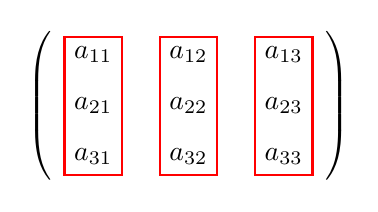
\begin{tikzpicture}[baseline=(mat.center)] % 基线对齐,矩阵排版不偏移
% 定义tikz矩阵,修正括号分隔符,精准保留原生圆括号
\matrix (mat) [matrix of math nodes,
               left delimiter=(,    % 左圆括号(正确写法)
               right delimiter=),   % 右圆括号(修正笔误,之前多写了()
               row sep=6pt,         % 行间距,适配3阶矩阵
               column sep=14pt]     % 列间距拉大,避免红色框互相重叠
{
  a_{11} & a_{12} & a_{13} \\  
  a_{21} & a_{22} & a_{23} \\  
  a_{31} & a_{32} & a_{33} \\
};
% 三列统一画红色框,thick让框更醒目,inner sep控制框与元素的间距
\draw[red, thick, inner sep=3pt] (mat-1-1.north west) rectangle (mat-3-1.south east); % 第一列红框
\draw[red, thick, inner sep=3pt] (mat-1-2.north west) rectangle (mat-3-2.south east); % 第二列红框
\draw[red, thick, inner sep=3pt] (mat-3-3.south east) rectangle (mat-1-3.north west); % 第三列红框
\end{tikzpicture}
\end{equation}
呃,这个,大家知道这个矩阵是怎么一回事吗?你当然可以把它看成一行一行的,也可以看成一列一列的,这个并不本质。这三个列分别代表什么?

大家应当是学过线性代数的啊!在这啊,我们要跟大家解释一下这个矩阵啊,和我们今天讲的$T(\delta (n-k))$这个东西,完全是一回事,你相信吗?原因在于我们矩阵就可以作为一个线性变换了,没问题吧?我们这个线性变换假如说也叫$T$,那么我这个$T$作用在这么一个向量上
\begin{equation}
\begin{pmatrix}  
  a_{11} & a_{12} & a_{13} \\  
  a_{21} & a_{22} & a_{23} \\  
  a_{31} & a_{32} & a_{33}  
\end{pmatrix} 
\begin{pmatrix}  
  x_{1}  \\  
  x_{2}  \\  
  x_{3}   
\end{pmatrix} 
\end{equation}
它作用在这个向量上就是,$x_1$乘上第一列,$x_2$乘上第二列,$x_3$乘上第三列,它为什么是这样的?想过吗?就是你在学线性代数的时候,你一定会学矩阵乘向量,这是一种运算法则,而老师会直接把这个运算法则告诉你,它一定就是这么个运算,但是它为什么是这样的呢?

这个原因就在我们今天讲的这个点上,我们来看看,实际上我们是想做这件事情
\begin{equation}
T \left (
\begin{pmatrix}  
  x_{1}  \\  
  x_{2}  \\  
  x_{3}   
\end{pmatrix} \right )
\end{equation}
对不对?我要用线性变换去对这样一个对象进行操作。那么,我们实际上是分两步的。第一步,我先把这个对象给分解了,我要把它分解成简单对象的叠加。这个分解啊,大家可能没意识,没意识的原因是什么呢?是因为坐标这个概念深入人心,从中学你就把这个概念深深地建立在脑子里了,因此你会觉得我们去做这么一件事
\begin{equation}
T \left (
\begin{pmatrix}  
  x_{1}  \\  
  x_{2}  \\  
  x_{3}   
\end{pmatrix} \right )=
T \left (
x_1
\begin{pmatrix}  
  1  \\  
  0  \\  
  0   
\end{pmatrix}+
x_2
\begin{pmatrix}  
  0  \\  
  1 \\  
  0   
\end{pmatrix}+
x_3
\begin{pmatrix}  
  0  \\  
  0  \\  
  1   
\end{pmatrix}
\right )
\end{equation}
因此你会觉得我们去做这么一件事,这个东西并没什么可说的!因为这个就是按坐标轴在做,但是实际上可能你忽略了一个重要的思想。我们在这里用到的是什么思想?是一种用简单对象表达复杂对象的思想,这个思想我们以后会经常用。其实你早就在用了,只是你没意识而已。就是,因为你会觉得坐标这个东西没有什么太多可说的,实际上这个东西也是用简单对象表达复杂对象,而且你现在这个坐标啊——这个简单对象的性质还好得不得了,因为你这个是一组正交的。以后大家会更有体会,如果我们用正交的对象进行分解,它给我们带来的优点会有多少。

好,假如是这样的话,这个事就变得简单了。因为我们会发现,由于它是线性的……注意!这个时候我还没矩阵呢,由于它是线性的,所以它自然就会写成这么个样子
\begin{equation}
\begin{aligned} 
T \left (
\begin{pmatrix}  
  x_{1}  \\  
  x_{2}  \\  
  x_{3}   
\end{pmatrix} \right )&=
T \left (
x_1
\begin{pmatrix}  
  1  \\  
  0  \\  
  0   
\end{pmatrix}+
x_2
\begin{pmatrix}  
  0  \\  
  1 \\  
  0   
\end{pmatrix}+
x_3
\begin{pmatrix}  
  0  \\  
  0  \\  
  1   
\end{pmatrix}
\right ) \\
&=
x_1 T \left (
\begin{pmatrix}  
  1  \\  
  0  \\  
  0   
\end{pmatrix}
\right )+
x_2 T \left (
\begin{pmatrix}  
  0  \\  
  1  \\  
  0   
\end{pmatrix}
\right )+
x_3 T \left (
\begin{pmatrix}  
  0  \\  
  0  \\  
  1   
\end{pmatrix}
\right )
\end{aligned} 
\end{equation}
这一点和矩阵没有半毛钱关系,我们在这用到的是线性性质。你看,我们强化自己对于线性的认识,因为这个概念会贯穿我们这一门课程,甚至会贯穿大家整个职业生涯。非线性的事太困难,我们通常不去碰,但线性的事我们要把它搞得手拿把攥才行。你现在线性的,你自然就有这样的分解,而此时我们看到了,什么东西自然就出现了呢?冲激响应!就是在你这里对应于冲激响应就是最后这三个量。
\begin{equation}
T \left (
\begin{pmatrix}  
  1  \\  
  0  \\  
  0   
\end{pmatrix}
\right ),\quad
T \left (
\begin{pmatrix}  
  0  \\  
  1  \\  
  0   
\end{pmatrix}
\right ),\quad
T \left (
\begin{pmatrix}  
  0  \\  
  0  \\  
  1   
\end{pmatrix}
\right )
\end{equation}
而今天我们讲到的其实比这要复杂,因为今天我们的冲激响应不止三个,咱们的冲激响应有无穷多个,那么你现在这里是有限维度的操作,因此你的冲激响应就三个。

这三个冲激响应很显然是需要特殊给予关注的,因此我们给他们了一套符号。我们令这个矩阵的第一列,就是第一个坐标分量的冲激响应
\begin{equation}
\begin{pmatrix}  
  a_{11}  \\  
  a_{21}  \\  
  a_{31}  
\end{pmatrix}=
T \left (
\begin{pmatrix}  
  1  \\  
  0  \\  
  0   
\end{pmatrix}
\right ),\quad
\begin{pmatrix}  
  a_{12}  \\  
  a_{22}  \\  
  a_{32}  
\end{pmatrix}=
T \left (
\begin{pmatrix}  
  0  \\  
  1  \\  
  0   
\end{pmatrix}
\right ),\quad
\begin{pmatrix}  
  a_{13}  \\  
  a_{23}  \\  
  a_{33}  
\end{pmatrix}=
T \left (
\begin{pmatrix}  
  0  \\  
  0  \\  
  1   
\end{pmatrix}
\right )
\end{equation}
然后令这个矩阵的第二列就是第二个坐标分量的冲激响应,第三列也一样。这么一来啊,我们的矩阵才算是出现了。你瞧瞧!你这么一来,它这个矩阵才会出现,因此——大家学过线性代数啊,大家对矩阵应当是有概念的——就是说,你矩阵里的列代表的实际上就是我们今天所讲到的冲激响应。

他为什么把它写成一个矩阵的样子呢?是因为它要把这些冲激响应强调出来,这东西是线性变换的核心。我们说线性变换,它输入做线性分解,得到输出也是线性叠加,线性叠加的基础是这些冲激响应。我们线性代数那自然是研究线性变换,而且是研究有限维欧式空间当中的线性变换,因此我们要强调出我们这个特殊的线性变换的冲激响应,我们怎么强调呢?
\begin{equation}
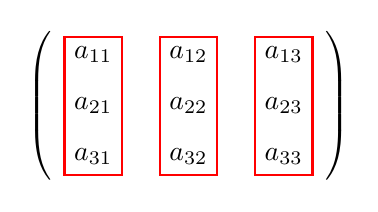
\begin{tikzpicture}[baseline=(mat.center)] % 基线对齐,矩阵排版不偏移
% 定义tikz矩阵,修正括号分隔符,精准保留原生圆括号
\matrix (mat) [matrix of math nodes,
               left delimiter=(,    % 左圆括号(正确写法)
               right delimiter=),   % 右圆括号(修正笔误,之前多写了()
               row sep=6pt,         % 行间距,适配3阶矩阵
               column sep=14pt]     % 列间距拉大,避免红色框互相重叠
{
  a_{11} & a_{12} & a_{13} \\  
  a_{21} & a_{22} & a_{23} \\  
  a_{31} & a_{32} & a_{33} \\
};
% 三列统一画红色框,thick让框更醒目,inner sep控制框与元素的间距
\draw[red, thick, inner sep=3pt] (mat-1-1.north west) rectangle (mat-3-1.south east); % 第一列红框
\draw[red, thick, inner sep=3pt] (mat-1-2.north west) rectangle (mat-3-2.south east); % 第二列红框
\draw[red, thick, inner sep=3pt] (mat-3-3.south east) rectangle (mat-1-3.north west); % 第三列红框
\end{tikzpicture}
\end{equation}
我们就把它排在这来作为强调!我们其实很想把$T\left ( x(n) \right ) = \sum\limits_{k=-\infty}^{+\infty}x(k)h(n,k)$这个东西排在这,但是这太多了,我们排不下。因此,我们只能这么写。

你看,我们今天所学到的知识,和我们在线性代数里早已经掌握的知识完全一致。它们处理的都是线性问题,它们都是做线性变换,它们都有相同的线性结构,它们的核心都是冲激响应,你看,没区别。的确没区别!如果大家对线性代数很熟悉,理解我们今天的这部分知识,那就没有任何的问题。

\subsubsection{Time-Invariant}\quad

好的,我们继续。我们从这继续

\begin{equation}
   T\left ( x(n) \right ) = \sum_{k=-\infty}^{+\infty}x(k)h(n,k)
\end{equation}
我们希望啊能够在线性的基础上,能够在线性的基础上再提一些要求。因为这个系统啊,它有不同的应用范围,有不同的针对对象,所以说我们时常对它有不同的要求。我们下面要提一个什么要求呢?叫做时不变(Time-Invariant)。

我们下面要提一个时不变的要求,什么意思?如果说,$x(n)$经过一个线性系统得到一个$y(n)$
\begin{equation}
   y(n) = T\left ( x(n) \right )
\end{equation}
那么,时不变的意思就是说,假如啊,我这个$x(n)$做了某种延时
\begin{equation}
   T\left ( x(n-n_d) \right )
\end{equation}
那么,我的$y(n)$也相应地有所变化,这个不奇怪!
\begin{equation}
   y(n-n_d) = T\left ( x(n-n_d) \right )
\end{equation}
我们对它的变化要有明确的规定,我们要求它的变化刚好也是这样的延时。这个东西叫时不变,它的不变性就体现在$x(n)$这个延迟做多少,$y(n)$这个延时也会相应地产生多少。

好的,我们来检查一下我们刚才所提到的两个典型的线性系统他们是不是时不变的。
\begin{itemize}
    \item 1.\quad Delay
\end{itemize}

一个是我们的延时器。延时器意味着我$y(n)$就等于$x(n-d)$
\begin{equation}
   y(n) = x(n-d)
\end{equation}
这是延迟器。如果我$x(n)$作某种延迟
\begin{equation}
   x(n) \longrightarrow x(n-n_d)
\end{equation}
那么就相当于
\begin{equation}
   x(n-d) \longrightarrow x(n-n_d - d)
\end{equation}
对吧!那么你这个$y(n)$就是
\begin{equation}
   y(n-n_d) = x(n-n_d-d)
\end{equation}
我们发现,这个东西的时不变特性,没有任何问题!好,我们接着来
\begin{itemize}
    \item 2.\quad Integration
\end{itemize}

如果我们考察一下积分器
\begin{equation}
   y(n) = \sum_{k=-\infty}^{n}x(k)
\end{equation}
那么,你同样$x(n)$作某种延迟的话,那这个地方就会是这个样子
\begin{equation}
   y(n) = \sum_{k=-\infty}^{n}x(k-n_d)
\end{equation}
好,我们要处理这个问题。其实它很简单,但是我们为什么在这故意写得很慢,是因为这个技巧大家要掌握——我们在这要用到一个计算技巧,它叫作换元。积分换元大家肯定很熟悉,相信大家的微积分基础一定很扎实!

那么,积分换元有三件事,哪三件事呢?我首先把所有的旧元换成新元,其次我要去做一下雅可比——就是我在旧元上去做的那个微元,要换成新元上做的微元,再其次我要改变积分限。积分限做适当处理,旧元新元它有个转换没问题吧!

求和换元和积分换元本质上是一样的,但是求和要简单,为什么呢?少一步,雅可比不用做了——微元的变化不用做了。剩下两个,我们挨个做。第一,把旧元换成新元
\begin{equation}
   k-n_d \longrightarrow k^{' }
\end{equation}
然后,第二,我们来处理这个求和上下限,下限不用说了,负无穷。上限是要改变的,因为你的$k$是从负无穷到$n$,那么你的$k^{' }$是$k-n_d$,很显然,这个
\begin{equation}
  \sum_{k=-\infty}^{n}x(k-n_d)\longrightarrow\sum_{k=-\infty}^{n-n_d}x(k^{' })
\end{equation}
而这个刚好等于
\begin{equation}
   y(n-n_d)=\sum_{k=-\infty}^{n-n_d}x(k^{' })
\end{equation}
没问题了!时不变!因为我$x$作为输入有一个什么样的延迟,$y$作为输出也就相应地有个什么样的延迟,所以这件事一定是时不变的。好的,我们继续啊。

\subsubsection{LTI(Linear Time-Invariant)}\quad

现在我们来考察,在时不变的情况下,我们的这样一个线性变换的基本结构
\begin{equation}
   T\left ( x(n) \right ) = \sum_{k=-\infty}^{+\infty}x(k)h(n,k)
\end{equation}
它会呈现出什么特殊的模样?我们已经是时不变了,时不变的意思就是说,你输入做一个什么样的动作,那么输出相应地也会做出动作,你输入做一个什么样的延迟,输出也会相应地做出一个什么样的延迟。好的,我们现在就来看一看啊。这意味着,如果我的输入做了一个延迟
\begin{equation}
   \sum_{k=-\infty}^{+\infty}x(k-n_d)h(n,k)
\end{equation}
这里是$k-n_d$了,然后我的冲激响应仍然是在这里,这是我的基础。那么,我现在来算一算这个求和,我们的计算跟刚才一模一样,我要做什么呢?我要做求和换元。我要把$k-n_d$换成$k'$,在目前这个情况下,换元很简单了,因为积分上下限是不用变的。你增加一个减少一个从你负无穷到正无穷,这个是不会有任何变化的。因此,你只需要把所有的旧元统统都换成新元就可以了,因此这里就变成
\begin{equation}
  \sum_{k=-\infty}^{+\infty}x(k-n_d)h(n,k)  \xrightarrow{k'=k-n_d}
  \sum_{k'=-\infty}^{+\infty}x(k')h(n,k'+n_d)
\end{equation}
好,那么我们现在希望怎么样?我们希望它做了这件事情以后,和我们没做之前相比,应当是什么样呢?假如这个东西是$y(n)$的话
\begin{equation}
   y(n) = \sum_{k=-\infty}^{+\infty}x(k)h(n,k)
\end{equation}
我们希望它等于$y(n-n_d)$
\begin{equation}
  y(n-n_d) \mathrel{\ooalign{$=$\cr\hidewidth\raisebox{-0.1ex}{$?$}\hidewidth\cr}} \sum_{k=-\infty}^{+\infty}x(k')h(n,k'+n_d)
\end{equation}
因为我$x$做了一个什么样的动作,相应地我希望$y$就能做出什么样的动作。那么这件事怎么能够做得到?我们应当说,有很多种方法来做到这一点,注意,不止一种。但是我们这里,强调一种我们最习惯的方法。怎么讲呢?看起来,我要对这个$h$做一下规定。如果我的$h$可以写成这样
\begin{equation}
   h(n,k) = h(n-k)
\end{equation}
你看,原本它是两个变元,我把它写成一个变元的样子。这个变元等于原来两个变元的差,如果我写成这个样子,你会发现,这个东西自然就变成
\begin{equation}
  \sum_{k=-\infty}^{+\infty}x(k-n_d)h(n-k)  \xrightarrow{k'=k-n_d}
  \sum_{k'=-\infty}^{+\infty}x(k')h(n-k'-n_d) = y(n-n_d)
\end{equation}
而这恰好是我们想要的结果。你可能还有别的方式,你有别的路数,能够确保我们这样的求和,可以写成$y$相应的延迟。当然啦!我们这里给出的是一个相对比较简单,我们也比较习惯的方式,因此看起来线性系统要想确保时不变,关键就在这
\begin{equation}
   h(n,k) = h(n-k)
\end{equation}
我们要把这一条单独拿出来说,因为如果有这一条的话,我们的线性系统就写成这么个样子
\begin{equation}
   y(n) = \sum_{k=-\infty}^{+\infty}x(k)h(n-k)
\end{equation}
而这个样子,这种运算,大家很熟悉了。这东西叫卷积(Convolution)。因此,我们强调为什么线性系统的输入输出关系可以写成卷积,两个条件,是两个条件共同作用的结果。一个是线性的,一个是时不变的,它是线性和时不变都有,我们才能写成卷积这么个样子。因此它也叫做LTI(Linear Time-Invariant),线性时不变。

\subsubsection{Convolution}\quad

卷积这个运算太好了,这个运算有多好,我们今天也许还体会不到,以后会反复体会。这也是为什么人们喜欢用线性系统的一个重要原因,是因为卷积这个操作,无论是从数学上还是从工程上,无论从理论上还是从数值上,它都有着大量的优点。如果我们能把线性系统线性时不变系统,把它局限在卷积上,这给我们带来的便利是非常非常多的。

好,我们要通过一个例子,让大家熟悉一下卷积操作。这个例子是奥本海姆书上的例子,很典型。我们希望用三种不同的方法来给大家熟悉一下卷积操作,因为这里涉及到了一个很重要的小技巧,叫做手算卷积。

手算卷积这个点啊,还算是一个比较重要的知识点,甚至是考点,因此大家一定要掌握。千万不要小看,手算卷积别说初学者了,学了半年以上的同学,如果没有足够的重视,没有足够的心理准备,都是算不对的。因为这件事真的不是那么简单,尽管它很初等,但不是那么简单。

好,我们的冲激响应首先给你
\begin{equation}
   h(n) = U(n) - U(n-N)
\end{equation}
然后呢,系统的输入也给了,我们通常都假定这个东西要收敛,要不然我们算不出结果
\begin{equation}
   x(n) = a^nU(n),\quad \left | a \right | <1
\end{equation}
给冲激响应,给系统输入,我们希望来计算系统的输出。根据我们刚才的说法,这个输出就是输入卷积冲激响应,没问题吧!
\begin{equation}
   y(n) = x(n)\circledast h(n)
\end{equation}
因此,它应当就是这个
\begin{equation}
\begin{aligned}
   y(n) &= x(n)\circledast h(n)\\
	&=\sum_{k=-\infty}^{+\infty}x(k)h(n-k)
\end{aligned}
\end{equation}
好了,再往下啊,就有意思了。那么,我们会发现,这个东西啊$h(n) = U(n) - U(n-N)$它只有一段。我们为什么说手算卷积,它往往不是那么容易算对呢,就是因为它都是一段一段的,一段一段的这件事就麻烦了。为什么,是因为你卷积这个操作,它需要从负无穷算到正无穷,那么从负无穷算到正无穷的时候,它这个一段一段的就有时候有,有时候没有。你得把什么时候有,什么时候没有看的特别清楚才可以。因此,我们现在来
\begin{equation}
\begin{aligned}
   y(n) &= x(n)\circledast h(n)\\
	&=\sum_{k=-\infty}^{+\infty}x(k)h(n-k)\\
   &=\sum_{k=-\infty}^{+\infty}a^kU(k)h(n-k)\\
	&=\sum_{k=-\infty}^{+\infty}a^kU(k)U(n-k) - \sum_{k=-\infty}^{+\infty}a^kU(k)U(n-N-k)
\end{aligned}
\end{equation}
你相信我,你一定要仔细地写,勿以善小而不为啊!你可能会觉得这东西我中学不就会了吗?会不会,你算出正确结果再说。好,我们到这稍微停一下,分析一下这个东西。

Analytical Solution

它有前面一部分,也有后面一部分,没错吧!前面一部分,要么得一,要么得零——我们暂且不看前面它的这个幅度调制这一块——那么,它要不得一,要不得零。所以我们就得分析了,分成几种情况
\begin{itemize}
    \item 1.\quad$n<0$
\end{itemize}

你第一项得一,是一个什么情况?你第一项得一的话,你这个$k$要大于等于零吧,$k\ge 0$,因为你得一,你$U(k)$得是一,$U(n-k)$也得是一,没问题吧!同时呢,你$k$要小于等于$n$,$k\le n$,这样你前头这一项才能是一。也就是$0 \le k \le n$。

后面这一项是一样的,你必须$k\ge 0$,同时呢$k\le n-N$。也就是$0 \le k \le n-N$。

这样一来,它前面得一,后面得一的情况,我们就给它分析清楚了。

先看前面这一条,如果$n<0$。在$n<0$的情况下,$k\ge 0$且$k\le n$就没法同时成立了。没问题吧!所以前面这一项就是零。

而如果$n<0$的话,你$n-N$就更负了,因此后面这条也不行。

所以,前后都是零。因此,这种情况下
\begin{equation}
   y(n) = 0 ,\quad n<0
\end{equation}
你$n<0$的时候,前一项得零,后一项也得零,因此这个$y(n)$只能是零。好,继续
\begin{itemize}
    \item 2.\quad$0 \le n \le N-1$
\end{itemize}

如果$n\ge 0$的话,前面一项就有东西了。但是呢,后一项大家看,后一项此时当$n \le N$的时候,它后一项还是零。因此第二个分界点,一定是在$N$上。

这种情况下,前面一项,没问题,是可以保留住的;但后一项根本保留不住。因此,这种情况下,这$k$是从$0$开始,因为你必须$k\ge 0$啊,一直到$n$
\begin{equation}
\begin{aligned}
   y(n) &= \sum_{k=0}^na^k,\quad 0 \le n \le N-1\\
&=\frac{1-a^{n+1}}{1-a}
\end{aligned}
\end{equation}
没问题吧!
\begin{itemize}
    \item 3.\quad$n \ge N$
\end{itemize}

第三种情况,如果$n$比这个大$N$,来得大,那这事,前一项不为零,后一项也不为零,但是它前后消不掉!因为你前后的这个起点终点啊,它不太一样。所以这种情况下,一共$N$项!
\begin{equation}
\begin{aligned}
   y(n) &= \sum_{k=0}^na^k - \sum_{k=0}^{n-N}a^k,\quad n \ge N\\
&=\sum_{k=n-N+1}^n a^k\\
&=a^{n-N+1}\frac{1-a^{N}}{1-a} 
\end{aligned}
\end{equation}
瞧瞧看!
\begin{equation}
\left\{\begin{aligned}
y(n) &= 0 ,\quad n<0\\
    y(n) &= \sum_{k=0}^na^k
=\frac{1-a^{n+1}}{1-a},\quad 0 \le n \le N-1
\\
    y(n) &= \sum_{k=0}^na^k - \sum_{k=0}^{n-N}a^k=\sum_{k=n-N+1}^n a^k=a^{n-N+1}\frac{1-a^{N}}{1-a} ,\quad n \ge N
\end{aligned}\right.
\end{equation}
如果我们要手算卷积,我们就要把它算得很清楚才行。大家可能觉得这个东西不够直观,的确,我们现在要用一个相对更直观的方法。

这就是我们想告诉大家的第二种方法,第二种方法是Graphical的。

Graphical Solution

那么,我们首先要把图给建立起来,这个图怎么说呢,这个是我的$h$

% 居中显示(极简版)
{\centering
\begin{tikzpicture}[
    >=Stealth, % 尖角箭头(贴合DSP绘图风格)
    axis/.style={thick, black}, % 坐标轴样式:粗黑线
    tick/.style={black, thin},  % 刻度线样式:细黑线
    label/.style={font=\small}, % 标注文字样式
    stem/.style={blue, thin},   % 垂直竖线(茎)样式:蓝色细线
    samp/.style={fill=blue, circle, size=2pt} % 采样点:蓝色实心圆
]
    % 1. 绘制坐标轴
    \draw[axis, ->] (-1, 0) -- (7, 0) node[right, label] {$n$};
    \draw[axis, ->] (0, -0.5) -- (0, 1.5) node[above, label] {$h(n)$};
    
    % 2. 绘制刻度(仅标注x轴0,保留所有刻度线)
    \foreach \x in {-1,0,1,2,3,4,5,6,7} {
        \draw[tick] (\x, 0.05) -- (\x, -0.05);
        \ifnum\x=0 \node[below, label] at (\x, -0.15) {$\x$};\fi
    }
    \foreach \y in {0,1} {
        \draw[tick] (0.05, \y) -- (-0.05, \y);
        \node[left, label] at (-0.15, \y) {$\y$};
    }

    % 核心新增:在x=5的位置标注n-N-1(放在x轴下方,不遮挡)
    \node[below, label, text=black] at (5, -0.3) {$n-N-1$};
    
    % 3. 绘制垂直竖线+采样点
    \foreach \n in {0,1,2,3,4,5} {
        \draw[stem] (\n, 0) -- (\n, 1);
        \fill[blue] (\n, 1) circle (2pt);
    }
    \fill[blue] (-1, 0) circle (2pt);
    \fill[blue] (6, 0) circle (2pt);
\end{tikzpicture}\par
}
那么,我们的$x$是这个样子,一个指数下降

% 居中显示
{\centering
\begin{tikzpicture}[
    >=Stealth, % 尖角箭头(DSP风格)
    axis/.style={thick, black}, % 坐标轴样式
    tick/.style={black, thin},  % 刻度线样式
    label/.style={font=\small}, % 标注文字样式
    stem/.style={blue, thin},   % 离散茎状线(蓝色细线)
    samp/.style={fill=blue, circle, size=2pt}, % 采样点(蓝色实心圆)
    envelope/.style={red, dashed, thick} % 包络线(红色虚线,粗一点突出)
]
    % 1. 定义指数衰减参数:a=0.6(保留计算逻辑,仅删除注释)
    \def\a{0.6} 
    
    % 2. 绘制坐标轴(核心修改:Y轴范围从-0.1→1.2 改为 -0.1→2.5,长度翻倍)
    % X轴(离散时间n):范围-1到9,带箭头,标注n(无修改)
    \draw[axis, ->] (-1, 0) -- (9, 0) node[right, label] {$n$};
    % Y轴(序列值x(n)):范围-0.1到2.5(原1.2→2.5,长度翻倍),带箭头,标注x(n)
    \draw[axis, ->] (0, -0.1) -- (0, 2.5) node[above, label] {$x(n)$};
    
    % 3. 绘制刻度(适配Y轴翻倍,新增1.5/2刻度)
    % X轴刻度(-1到9,仅标注0)(无修改)
    \foreach \x in {-1,0,1,...,9} {
        \draw[tick] (\x, 0.05) -- (\x, -0.05); % 刻度线
        \ifnum\x=0 \node[below, label] at (\x, -0.15) {$\x$};\fi
    }
    % Y轴刻度(0/0.5/1/1.5/2,适配两倍长度的轴)
    \foreach \y in {0,0.5,1,1.5,2} {
        \draw[tick] (0.05, \y) -- (-0.05, \y); % 刻度线
        \node[left, label] at (-0.2, \y) {$\y$};
    }
    
    % 4. 绘制离散序列:茎状线+采样点(n=0~8)(无修改)
    \foreach \n in {0,1,...,8} {
        \pgfmathparse{\a^\n} 
        \let\xn\pgfmathresult 
        \draw[stem] (\n, 0) -- (\n, \xn); % 茎状线
        \fill[blue] (\n, \xn) circle (2pt); % 采样点
    }
    
    % 5. 绘制指数包络线(无修改)
    \draw[envelope] plot[smooth, domain=0:8] (\x, {\a^\x});
\end{tikzpicture}\par
}
下面我们要看一下这个卷积
\begin{equation}
\begin{aligned}
   y(n) &= x(n)\circledast h(n)\\
   &=\sum_{k=-\infty}^{+\infty}x(k)h\bigl(
     % 核心:inner sep从0.5pt增至1.5pt,框体明显变大;thick保持红线粗细
     \tikz[baseline=(n.base)]{\node[draw=red, thick, inner sep=1.5pt] (n) {$n$};}
     -k\bigr)
\end{aligned}
\end{equation}
这个东西它不是特别好看,原因在哪呢?就是你的求和变量是$k$,可是这个地方一上来是$n$不是$k$啊。初学的时候,我们就容易把这个事看得有点眼晕,我们教大家一招。就是你把这个$h(n-k)$做一下改写,把它改写成这个
\begin{equation}
   h(n-k) = h(-(k-n))
\end{equation}
我们为什么要这么做?这么做的原因是,为了把前后这两项都搞成以$k$为主导。这么一来,我们两者之间的对应,会更加清楚。搞成这样之后,大家就会知道了,这首先是$h(-k)$,然后左正右负,左加右减。这个大家中学都学过啊,减$n$它是向右移动。那么如果$n$是大于零的,它是向右移动;如果$n$是小于零的,它是向左移动。因此,我们现在明确了一个点,我们画一个稍微大一点的图

% 居中显示,宽度≤A4
{\centering
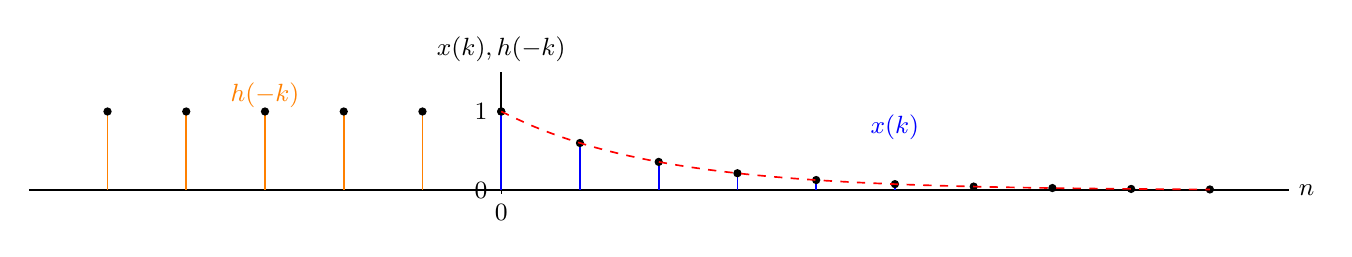
\begin{tikzpicture}[
    scale=1,
    every node/.style={font=\small}, % 统一字体大小
    axis/.style={thick, black, >=Stealth}, % 坐标轴(保持粗线,适配整体)
    tick/.style={black, thin}, % 刻度线(细线条,不抢视觉)
    hseq/.style={orange, semithick}, % h(-n)茎状线:从thin改semithick(加粗)
    xseq/.style={blue, semithick},   % x(n)茎状线:从thin改semithick(加粗)
    samp/.style={fill=black, circle, radius=1.5pt} % 采样点:从1pt改1.5pt(放大)
]
    % 1. 绘制坐标轴(x轴-6~10,y轴0~1.5,适配A4)
    \draw[axis] (-6, 0) -- (10, 0) node[right] {$n$};
    \draw[axis] (0, 0) -- (0, 1.5) node[above] {$x(k), h(-k)$};
    
    % 2. 刻度:仅保留0
    \foreach \x in {0} {
        \draw[tick] (\x, 0.05) -- (\x, -0.05) node[below] {$\x$};
    }
    % Y轴刻度:0,1
    \foreach \y in {0,1} {
        \draw[tick] (0.05, \y) -- (-0.05, \y) node[left] {$\y$};
    }

    % 3. 绘制h(-n)(n=-5~0,值为1)
    \foreach \n in {-5,-4,-3,-2,-1,0} {
        \draw[hseq] (\n, 0) -- (\n, 1);
        \fill[samp] (\n, 1) circle (1.5pt); % 采样点放大到1.5pt
    }
    % 负半轴上方标注h(-n)
    \node[orange, font=\small] at (-3, 1.2) {$h(-k)$};

    % 4. 绘制x(n)=0.6ⁿU(n)(n=0~9)
    \foreach \n in {0,1,...,9} {
        \pgfmathparse{0.6^\n}
        \let\xn\pgfmathresult
        \draw[xseq] (\n, 0) -- (\n, \xn);
        \fill[samp] (\n, \xn) circle (1.5pt); % 采样点放大到1.5pt
    }
    % x(n)包络线:从thin改semithick(加粗)
    \draw[red, dashed, semithick] plot[smooth, domain=0:9] (\x, {0.6^\x});
    % 正半轴上方标注x(n)
    \node[blue, font=\small] at (5, 0.8) {$x(k)$};

\end{tikzpicture}\par
}
你看,我们的$x$在这。我们的$h$,但是有个负号它就颠倒过来了,这就是我们很多教科书上面所说的倒转求和。它要到转过来,就是出于对这个负号的考虑。然后倒转过来之后,它不是还要平移吗。你既然一平移,大家立马就看出来了,这要比我们刚才纯解析的分析要直观得多——我们立马就看出来三种情况,一定是三种情况。

% 居中显示,宽度≤A4
{\centering
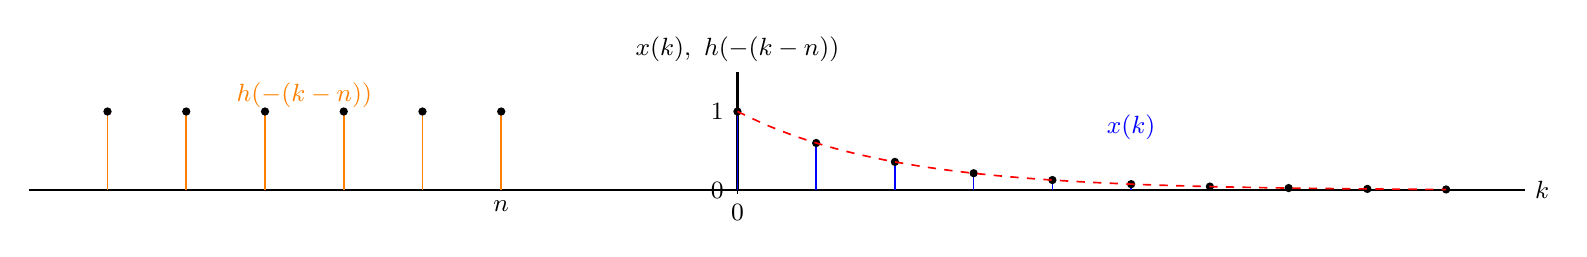
\begin{tikzpicture}[
    scale=1,
    every node/.style={font=\small}, % 统一字体
    axis/.style={thick, black, >=Stealth}, % 坐标轴(粗线+尖角箭头)
    tick/.style={black, thin}, % 刻度线(细线条)
    hseq/.style={orange, semithick}, % h(-(k-n))茎状线(加粗)
    xseq/.style={blue, semithick},   % x(k)茎状线(加粗)
    samp/.style={fill=black, circle, radius=1.5pt} % 采样点(放大到1.5pt)
]
    % 1. 绘制坐标轴(x轴-9~10,变量改为k,y轴0~1.5)
    \draw[axis] (-9, 0) -- (10, 0) node[right] {$k$}; % 替换n→k
    \draw[axis] (0, 0) -- (0, 1.5) node[above] {$x(k),\ h(-(k-n))$}; % 替换+修改h标注

    % 2. 刻度:仅保留0(变量仍为k)
    \foreach \x in {0} {
        \draw[tick] (\x, 0.05) -- (\x, -0.05) node[below] {$\x$};
    }
    % Y轴刻度:0,1
    \foreach \y in {0,1} {
        \draw[tick] (0.05, \y) -- (-0.05, \y) node[left] {$\y$};
    }

    % 3. 绘制左移的h(-(k-n))(k=-8~-3,值为1,最右侧点k=-3)
    \foreach \k in {-8,-7,-6,-5,-4,-3} { % 循环变量替换n→k(内部索引,不显示)
        \draw[hseq] (\k, 0) -- (\k, 1); % 橙色加粗茎状线
        \fill[samp] (\k, 1) circle (1.5pt); % 放大的采样点
    }
    % 标注h(-(k-n))(左移后的中间位置:x=-5.5, y=1.2)
    \node[orange, font=\small] at (-5.5, 1.2) {$h(-(k-n))$};
    % 在h序列最右侧点(k=-3)的x轴下方标注n
    \node[black, font=\small] at (-3, -0.2) {$n$};

    % 4. 绘制x(k)=0.6ᵏU(k)(k=0~9,变量替换n→k)
    \foreach \k in {0,1,...,9} { % 循环变量替换n→k
        \pgfmathparse{0.6^\k}
        \let\xk\pgfmathresult
        \draw[xseq] (\k, 0) -- (\k, \xk); % 蓝色加粗茎状线
        \fill[samp] (\k, \xk) circle (1.5pt); % 放大的采样点
    }
    % x(k)包络线(加粗虚线)
    \draw[red, dashed, semithick] plot[smooth, domain=0:9] (\x, {0.6^\x});
    % 标注x(k)(原位:x=5, y=0.8,替换n→k)
    \node[blue, font=\small] at (5, 0.8) {$x(k)$};

\end{tikzpicture}\par
}

一种情况是它移动到这来了,因为这个点刚好是$n$,没错吧!你$n=0$的时候,两边刚好踩在一起,如果这个$n<0$的时候,它就挪开了。因为$n$是负的情况下,你减一个$n$相当于是向左移,在这里,这两个东西根本重叠不上!而第二种情况呢,它往右动

% 居中显示,宽度≤A4
{\centering
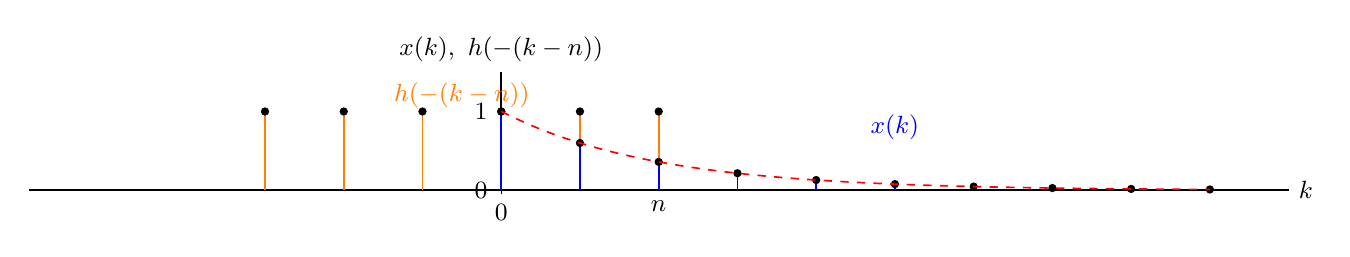
\begin{tikzpicture}[
    scale=1,
    every node/.style={font=\small}, % 统一字体
    axis/.style={thick, black, >=Stealth}, % 坐标轴(粗线+尖角箭头)
    tick/.style={black, thin}, % 刻度线(细线条)
    hseq/.style={orange, semithick}, % h(-(k-n))茎状线(加粗)
    xseq/.style={blue, semithick},   % x(k)茎状线(加粗)
    samp/.style={fill=black, circle, radius=1.5pt} % 采样点(放大到1.5pt)
]
    % 1. 绘制坐标轴(x轴-6~10,适配平移后的h,y轴0~1.5)
    \draw[axis] (-6, 0) -- (10, 0) node[right] {$k$}; 
    \draw[axis] (0, 0) -- (0, 1.5) node[above] {$x(k),\ h(-(k-n))$};

    % 2. 刻度:仅保留0
    \foreach \x in {0} {
        \draw[tick] (\x, 0.05) -- (\x, -0.05) node[below] {$\x$};
    }
    % Y轴刻度:0,1
    \foreach \y in {0,1} {
        \draw[tick] (0.05, \y) -- (-0.05, \y) node[left] {$\y$};
    }

    % 3. 绘制右移的h(-(k-n))(k=-3~2,部分在左侧、部分与x重合)
    % 左侧:k=-3~-1;重合区:k=0~2 → 部分重叠,未完全重合
    \foreach \k in {-3,-2,-1,0,1,2} { 
        \draw[hseq] (\k, 0) -- (\k, 1); % 橙色加粗茎状线
        \fill[samp] (\k, 1) circle (1.5pt); % 放大的采样点
    }
    % 标注h(-(k-n))(平移后的中间位置:x=-0.5, y=1.2,不挡重叠区)
    \node[orange, font=\small] at (-0.5, 1.2) {$h(-(k-n))$};
    % 在h序列最右侧点(k=2)的x轴下方标注n(同步右移)
    \node[black, font=\small] at (2, -0.2) {$n$};

    % 4. 绘制x(k)=0.6ᵏU(k)(k=0~9,原位不动)
    \foreach \k in {0,1,...,9} {
        \pgfmathparse{0.6^\k}
        \let\xk\pgfmathresult
        \draw[xseq] (\k, 0) -- (\k, \xk); % 蓝色加粗茎状线
        \fill[samp] (\k, \xk) circle (1.5pt); % 放大的采样点
    }
    % x(k)包络线(加粗虚线)
    \draw[red, dashed, semithick] plot[smooth, domain=0:9] (\x, {0.6^\x});
    % 标注x(k)(原位:x=5, y=0.8)
    \node[blue, font=\small] at (5, 0.8) {$x(k)$};

\end{tikzpicture}\par
}
你动了一部分过来,注意,$n$在这里。所以两边重合的部分,是零到$n$,很直观吧!好,再往下,它继续往右动,然后它就变成这个样子了,全重叠进来了。

% 居中显示,宽度≤A4
{\centering
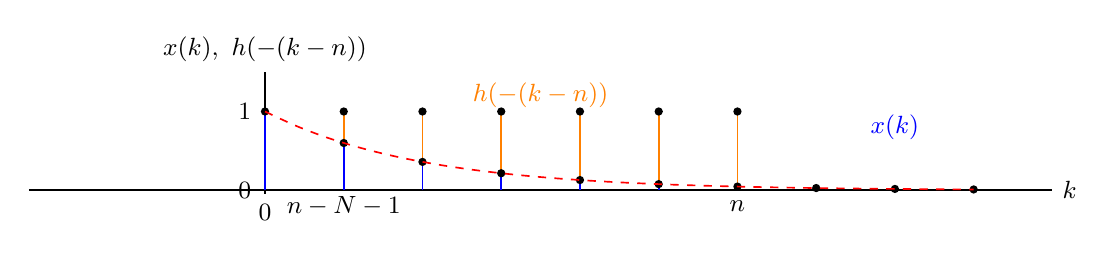
\begin{tikzpicture}[
    scale=1,
    every node/.style={font=\small}, % 统一字体
    axis/.style={thick, black, >=Stealth}, % 坐标轴(粗线+尖角箭头)
    tick/.style={black, thin}, % 刻度线(细线条)
    hseq/.style={orange, semithick}, % h(-(k-n))茎状线(加粗)
    xseq/.style={blue, semithick},   % x(k)茎状线(加粗)
    samp/.style={fill=black, circle, radius=1.5pt} % 采样点(放大到1.5pt)
]
    % 1. 绘制坐标轴(x轴-3~10,适配右挪后的h,y轴0~1.5)
    \draw[axis] (-3, 0) -- (10, 0) node[right] {$k$}; 
    \draw[axis] (0, 0) -- (0, 1.5) node[above] {$x(k),\ h(-(k-n))$};

    % 2. 刻度:仅保留0
    \foreach \x in {0} {
        \draw[tick] (\x, 0.05) -- (\x, -0.05) node[below] {$\x$};
    }
    % Y轴刻度:0,1
    \foreach \y in {0,1} {
        \draw[tick] (0.05, \y) -- (-0.05, \y) node[left] {$\y$};
    }

    % 3. 绘制右挪一格的h(-(k-n))(k=1~6,左端k=1,右端k=6)
    \foreach \k in {1,2,3,4,5,6} { 
        \draw[hseq] (\k, 0) -- (\k, 1); % 橙色加粗茎状线
        \fill[samp] (\k, 1) circle (1.5pt); % 放大的采样点
    }
    % 标注h(-(k-n))(序列中间位置:x=3.5, y=1.2,不挡图像)
    \node[orange, font=\small] at (3.5, 1.2) {$h(-(k-n))$};
    % 在h左端(k=1)下方标注n-N-1
    \node[black, font=\small] at (1, -0.2) {$n-N-1$};
    % 在h右端(k=6)下方标注n(同步右挪)
    \node[black, font=\small] at (6, -0.2) {$n$};

    % 4. 绘制x(k)=0.6ᵏU(k)(k=0~9,原位不动)
    \foreach \k in {0,1,...,9} {
        \pgfmathparse{0.6^\k}
        \let\xk\pgfmathresult
        \draw[xseq] (\k, 0) -- (\k, \xk); % 蓝色加粗茎状线
        \fill[samp] (\k, \xk) circle (1.5pt); % 放大的采样点
    }
    % x(k)包络线(加粗虚线)
    \draw[red, dashed, semithick] plot[smooth, domain=0:9] (\x, {0.6^\x});
    % 标注x(k)(避开重叠区:x=8, y=0.8)
    \node[blue, font=\small] at (8, 0.8) {$x(k)$};

\end{tikzpicture}\par
}

而此时,这里是$n$,这里是$n-N-1$,一目了然。我们需要做的,刚好就是从$n-N-1$到$n$来做求和。我们相当于是把刚才的这个解析过程,用很直观的图给大家显示出来,因此这也是手算卷积的一个重要的技巧——所谓用图来求解。这个东西,大家可以根据你的喜好随意地选择。你可以做解析的,因为有的同学你可能做解析更习惯;你也可以作图,因为有的同学可能直观思维比较好,所以他对图更加地有认识。无论用哪一个,都可以做出正确结果。手算卷积一定是我们这门课的重要的一个知识点。

这个东西不存在不会的问题,只存在你对它不重视,你觉得这玩意儿手拿把攥,你觉得这东西不都是中学做的计算吗,你看这里头有一点微积分的意思吗。但是,算对,再来说话。

我们再提供大家一个路子,咱们同学还算是比较高水平的同学啊,我们不要觉得这是小事,就不以为然。之所以这个手算卷积,会让你有一点感觉头疼,其实很主要的原因就是因为它都是一段一段的。就是如果它没有一段一段的,它全是连续的,那么它这个手算卷积的话就要相对简单很多了。因此,我们在这给大家这么一个东西。

General Solution

就是$x(n)$就等于
\begin{equation}
    x(n) = a(n)U(n)
\end{equation}
然后
\begin{equation}
    h(n) = b(n)U(n-N)
\end{equation}
我们给一个一般性的结果,那么根据定义,它就是这个
\begin{equation}
\begin{aligned}
   y(n) &= x(n)\circledast h(n)\\
&= \sum_{k=-\infty}^{+\infty}x(k)h(n-k)\\
&= \sum_{k=-\infty}^{+\infty}a(k)b(n-k)U(k)U(n-N-k)
\end{aligned}
\end{equation}
这个和刚才其实是一回事。你看,我们同样是分析这个东西$U(k)U(n-N-k)$,我们要求$0 \le k \le n-N$,没问题吧!所以这个东西$U(k)U(n-N-k)$要不是$\ge 0$,要不就$\le 0$。如果是小于等于零,那它啥也没有;如果它大于等于零的话,那么这个结果就来了
\begin{equation}
\begin{aligned}
   y(n) &= x(n)\circledast h(n)\\
&= \sum_{k=-\infty}^{+\infty}x(k)h(n-k)\\
&= \sum_{k=-\infty}^{+\infty}a(k)b(n-k)U(k)U(n-N-k)\\
&=\left ( \sum_{k=0}^{n-N}a(k)b(n-k) \right )U(n-N) 
\end{aligned}
\end{equation}
因为我只有在$n-N \ge 0$的时候它才有值,而小于零,它是没有值的。好!所以这是一个某种意义上具有一般性的结果,那么我们把这个结果用到咱们这个例子里来啊。那我立刻就能得到
\begin{equation}
   y(n) = \left ( \sum_{k=0}^n a^k \right )U(n) - \left ( \sum_{k=0}^{n-N} a^k \right )U(n-N)
\end{equation}
你可以仔细检查,这两项一减出来就是我们这个结论,没差别。因此,现在咱们相当于有三个路子,一个路子是解析硬算,一个路子是用图帮助分析。还有一个路子,如果我们的问题都是出在各种各样的$U$上,我们就可以先把和$U$有关的这个卷积算清楚,然后我们来直接代公式。哪一个你用得最熟,哪一个你觉得最保险,你觉得哪一个是你心目中的黄金路径,你就用谁。

\subsubsection{Causal(Physically Realizable)}\quad

好,我们继续。有了卷积这个结果,我们就可以进一步地探讨线性变换和线性系统中,的一个还挺有用的性质,叫因果性(Causal)。什么叫因果?因果也有一个说法,叫作物理可实现(Physically Realizable)。

什么是因果呢?通俗地讲,就是说我在输出$y$的时候,我所用到的$x$它的时间不能比我$y$的输出时间更靠后。你想想看,这个东西应该是个起码的要求吧!你作为一个系统而言,你$n$时刻的输出,怎么可能用到$n+1$时刻的输入——$n+1$时刻还没到呢!你能用到的除了$n$时刻本身的输入以外,顶多顶多再往前用,没问题吧!因此就是说,它只依赖于$n$时刻之前的这些$x$
\begin{equation}
   y(n) = T\left ( x(n),x(n-1),x(n-2),\cdots \right )
\end{equation}
这个东西叫因果。如果我有这个要求,再结合我们的卷积,就很容易地知道我们要怎样求冲激响应。冲激响应是我们线性系统的关键啊!我对线性系统所有的条件,理论上来讲,它都要体现在冲激响应上。如果这是线性时不变系统,它又是个卷积了,那么它这个冲激响应就更有特点。我们加上因果的限制,冲激响应需要怎么样呢
\begin{equation}
   h(n) = 0,\quad n < 0
\end{equation}
冲激响应需要满足这么个条件。你想啊,我现在相当于只能加到$n$,没错吧!
\begin{equation}
\begin{aligned}
   y(n) &= x(n)\circledast h(n)\\
&= \sum_{k=-\infty}^{n}x(k)h(n-k)\\
\end{aligned}
\end{equation}
我只能加到$n$,那么我加到$n$以后,你看看,真正起作用的冲激响应只有正半轴。你如果说负半轴有值,那就意味着某一个$k<0$这个冲激响应都有值,那么我就意味着,我用到的已经是$x(n)$之后的结果。所以,这是因果性。

好,我们可以从另一个角度来看。换个角度
\begin{equation}
   y(n) = \sum_{k=-\infty}^{+\infty}x(k)h(n-k)
\end{equation}
这是我们的卷积,这个卷积是可以交换次序的。怎么交换次序?求和换元就可以了。你看,我令$k' = n-k$没问题吧!
\begin{equation}
   y(n) = \sum_{k=-\infty}^{+\infty}x(k)h(n-k)\xrightarrow{k'=n-k}y(n) = \sum_{k'=-\infty}^{+\infty}x(n-k')h(k')
\end{equation}
如果这个$k' = n-k$这样换的话,那么就有$k = n-k'$,然后我们的积分限不会变的——其实积分限是变了,变成什么了呢,变成正无穷到负无穷了,但是这不重要,这不是积分。这是求和,求和的话,你从正加到负和从负加到正是完全一样的;而积分的话,你是要颠倒一下次序的,颠倒次序要加一个负号,但这个负号会被消掉——会被什么消掉——你前面的微元。也会出一个负号!两个负号是会被消掉的。因此
\begin{equation}
\begin{aligned}
   y(n) &= \sum_{k=-\infty}^{+\infty}x(k)h(n-k)\\
&= \sum_{k=-\infty}^{+\infty}x(n-k)h(k)
\end{aligned}
\end{equation}
你从这件事上看因果,会看得更明白。我们要求,一定是这个$k$,要大于等于零才行。这个时候,实际上因果相当于是你这里求和只能从零开始
\begin{equation}
   y(n) = \sum_{k=0}^{+\infty}x(n-k)h(k)
\end{equation}
你$k \ge 0$,你才能确保这里$x$的时间都是在$n$之前。因此,你剩下的冲激响应通通都在正半轴上。如果你但凡有一个$k\le0$,冲激响应不为零的话,这就意味着你的$y$当中包含有$n$时刻之后的$x$,那么这就肯定不是因果的了。

\subsubsection{Stability}\quad

好,还有一个条件也被提及。但是这个事我们很少讨论,所以我们给大家提一嘴就行了,所谓的稳定性。

那么稳定性的意思是说,你如果$x$是有界的
\begin{equation}
   \left | x(n) \right | \le C_x,\quad \forall n \quad\Longrightarrow \quad\left | y(n) \right | \le C_y,\quad \forall n
\end{equation}
我一定可以推出,这个$y$也是有界的。实际上确保稳定性的充分条件有很多,这绝对不止一个两个。我们这里给出的是最简单的一个,就是假如我有这一条
\begin{equation}
   \sum_{k=-\infty}^{+\infty}\left | h(k) \right | \le C_h,\quad \forall n 
\end{equation}
假如我们有这一条,那就一定有稳定性。这个很简单啊,那么我们只要做一个简单的放缩就行了,因为你现在有卷积
\begin{equation}
   \left | y(n) \right | = \left | \sum_{k=-\infty}^{+\infty}h(k)x(n-k) \right |
\end{equation}
我们为什么要一遍一遍地写这件事,大家好像觉得哎哟好像没什么必要——重复是最好的练习。你写熟了,写顺溜了,写习惯了,这东西就会印在你脑子里;否则的话,过眼云烟。什么叫过眼云烟,看一遍就走了,一定是过眼云烟。所以我们强调一定要写。哎它一定小于等于这个
\begin{equation}
\begin{aligned}
   \left | y(n) \right | &= \left | \sum_{k=-\infty}^{+\infty}h(k)x(n-k) \right |\\
&\le \sum_{k=-\infty}^{+\infty}\left |h(k)\right |\left |x(n-k) \right |
\end{aligned}
\end{equation}
因为你后头这一部分是$\left |x(n-k) \right |\le C_x$的,所以我们把它提出来
\begin{equation}
\begin{aligned}
   \left | y(n) \right | &= \left | \sum_{k=-\infty}^{+\infty}h(k)x(n-k) \right |\\
&\le \sum_{k=-\infty}^{+\infty}\left |h(k)\right |\left |x(n-k) \right |\\
&\le C_x\sum_{k=-\infty}^{+\infty}\left |h(k)\right |\\
&\le C_xC_h\\
&=C_y
\end{aligned}
\end{equation}
大家的数学训练,看这种东西那简直是张飞吃豆芽了,但是勿以善小而不为。那么我们定义最后为$C_y$就可以了。这就是我们说的稳定性。

\subsubsection{Summary}\quad

好的,我们总结一下。我们今天重点学到了两部分知识。

一部分是离散的信号,这一部分我们简单提一下,最关键的一点在于我们知道了什么叫做分解——用冲激来进行分解。

第二部分知识是离散的线性系统。我们重点学到了什么呢?重点学到了线性系统的两个非常关键的点。第一,冲激响应。冲激响应是线性系统输出的基石,是它输出的组合的原材料。因为线性确保了我们输入如果被分解好了,输出同样是可以写成叠加的样子。因此,我们把冲激响应要深深地印在脑海里。这是我们理解线性系统的关键。这个概念并不新,我们学过线性代数,我们知道矩阵,我们知道矩阵的列,矩阵的列就是冲激响应,没有任何不同。只不过它的冲激响应有限维的,因此我们就把它排在那了,你说这多笨。这个显得很笨的样子。我们通常的这种系统的冲激响应,都是无穷多维的,无穷多维的话我们就没必要把它排在那了,那么我们用一个符号来表达它就OK了。此其一。

其二,时不变。如果加上时不变,这个系统的输出就是输入与冲激响应的卷积了。卷积运算要熟练地掌握,手算卷积也是每一位同学应当经历过的东西。

除了这两条之外,我们还有两个简单的线性系统的性质。一个是因果的,一个是稳定的,这个在今后的学习当中,我们有可能会提及,OK我们今天就到这吧!

\newpage
\section{Discrete Signal and Discrete System \uppercase\expandafter{\romannumeral 2}}\quad

好,我们开始上课啊。今天我们要继续学习离散信号和系统。那么信号与系统大家都已经有概念了,对于连续的信号与系统,相信大家都已经很好地掌握了。那么我们希望从离散的角度帮助大家把这些基本概念再重新复习一下。

那么上一堂课,我们讲到的是时域特性,今天呢我们会讲频域的。

\subsection{Frequency Domain}\quad

我们学习信号与系统这个课程,最大的一个收获就在于懂得怎么样从时域和频域两个角度来理解信号,并且来理解系统。事实上,时域和频域它是一块石头的两个面,我们作为信号处理工程师,是要具有时域频域两种眼光的。

\subsubsection{Transition Function}\quad

我们首先来谈论一个问题,就是说对于一个线性系统而言,假设我现在有一个离散信号
\begin{equation}
    \left \{ x(n) \right \} \longrightarrow 
    % 绘制包含L的方框:基线对齐+紧凑方框
    \tikz[baseline=(Lbox.base)]{\node[draw=black, inner sep=4pt] (Lbox) {$L$};}
    \longrightarrow \left \{ y(n) \right \}
\end{equation}
这是一个时域上的离散信号。那么,我这个离散信号啊,希望能够通过一个线性系统得到某个输出。这个线性系统啊,它对于我离散信号的作用啊,我当然不好说它一定能把我怎么样。因为它的这个作用从我们上一节课得到的知识来看呢,它属于是一个卷积。
\begin{equation}
   L\left ( x(n) \right ) = \sum_{k=-\infty}^{+\infty}h(k)x(n-k) 
\end{equation}
我们现在很感兴趣——我的信号是一个什么样的结构,使得它这个卷积输出啊,就能够有一个让我们非常满意的结果。什么样的结果呢?就是说,我对$x(n)$进行作用以后,我通过这样的卷积操作,我们希望仍然得到的是一个和$x(n)$相关的东西
\begin{equation}
   L\left ( x(n) \right ) = \sum_{k=-\infty}^{+\infty}h(k)x(n-k) = H\cdot x(n)
\end{equation}
换句话说,是一个线性因子$H$再乘上$x(n)$。我希望得到这么一个结果,这个结果大家一点都不陌生。
\begin{equation}
   Ax = \lambda x
\end{equation}
因为类似这样的结果,大家在线性代数里是学过的。那么我们一个矩阵作用在某一个矢量上,我们讲假如我们得到的结果仍然是这个矢量本身,只是对这个矢量进行了一下尺度变换,进行了一下线性操作,我们就称这个矢量是什么呢?我们就称它是我们这个矩阵的特征矢量(Eigen-vector)。这是我们在线性代数里已经建立起来的概念。

而今天呢,我们希望能够把这个概念给延伸到我们的线性系统上。因为线性代数里,我们的线性变换也是一种线性系统,只不过这个线性系统它是有限维的而已。而我们今天面对的是相对复杂的,无限维的线性系统,但是我们仍然希望能够把特征矢量这个概念延伸过来。那问题就来了,什么样的$x(n)$它具有这样的特性,可以成为线性系统的特征矢量?应当讲,线性系统的特征矢量,这个品种还是很多的,其中很典型的有一种。就是这一种
\begin{equation}
   x(n) = a^n
\end{equation}
你先甭管这个$a$是什么,我们来看一看,如果$x(n)$是$a$的$n$次方,我们会得到什么?那么这样一来,我作用在$a^n$上就会有一个卷积,这个卷积就会呈现出这么一个模样
\begin{equation}
   L\left ( a^n \right ) = \sum_{k=-\infty}^{+\infty}h(k)a^{n-k}
\end{equation}
我们把这个东西稍微整理一下啊,它可以把$a^n$从中提出来,提出来之后就可以得到
\begin{equation}
\begin{aligned}
   L\left ( a^n \right ) &= \sum_{k=-\infty}^{+\infty}h(k)a^{n-k}\\
&= \left ( \sum_{k=-\infty}^{+\infty}h(k)a^{-k} \right )a^n
\end{aligned}
\end{equation}
就是这么一个结果。我们可以进一步引入一个符号,把前面这一部分写成这个样子
\begin{equation}
\begin{aligned}
   L\left ( a^n \right ) &= \sum_{k=-\infty}^{+\infty}h(k)a^{n-k}\\
&= \left ( \sum_{k=-\infty}^{+\infty}h(k)a^{-k} \right )a^n\\
&= H(a)\cdot a^n
\end{aligned}
\end{equation}
因为前面这一部分确实是依赖于$a$的。这样一来啊,我们有了一个感觉——原本在矩阵当中,我们已经得到的特征矢量的概念,看起来可以很自然地延伸到我们的线性系统当中来——只要我们能够取我们的线性系统输入为$a^n$,那么这个输出啊,刚好就可以让我们看到特征的影子。因为$a^n$仍然在,没有变!你看它一点都没有变,而前面呢确实有了一个因子$H(a)$,这个因子与$a$是有关的,但是呢它并没有显式地依赖于$a^n$,特别是它并没有显式地依赖于这个$n$。因此,特征在这里体现出来了。我们管这个东西,叫做特征函数(Eigen-function)。在线性代数里面我们有特征矢量,那是对有限维而言;现在,我们有了特征函数,这是对于一般的无限维的线性系统。

这个特征函数,还没有让我们满意。因为它没有明确的物理含义,我们现在要给它赋予明确的物理含义。我们已经有这样的经验了,我们知道什么样的东西是有明确物理含义的呢?简谐振动。简谐振动意味着我们可以用复指数来进行刻画,而如果我们给这个$a$赋予明确的物理含义,这事儿就简单了。
\begin{equation}
   a = e^{j \omega}
\end{equation}
你看,这么一来,你$a$的$n$次方就好办了
\begin{equation}
   a = e^{j \omega}\quad \Longrightarrow \quad a^n = e^{j\omega n}
\end{equation}
这就是简谐振动。而一写到这里,大家立马就感觉到了,这个东西我们一点都不陌生。这个东西它关联着傅里叶变换,这也使得我们一下子将傅里叶变换与我们线性系统的特征函数联系到了一起,因为代表着简谐振动的复指数函数,它刚好就是我们线性系统的特征函数。

因此现在我们就能够对这个系统啊,进行一番新的描述了。因为我们线性系统,作用在简谐振动上,我们就可以把刚才的结果用上来
\begin{equation}
   L\left (  e^{j\omega n} \right ) =  \left (  \sum_{k=-\infty}^{+\infty}h(k)e^{-j\omega k} \right )\cdot e^{j\omega n}
\end{equation}
因此,我们可以再引入一个符号
\begin{equation}
\begin{aligned}
   L\left (  e^{j\omega n} \right ) &=  \left (  \sum_{k=-\infty}^{+\infty}h(k)e^{-j\omega k} \right )\cdot e^{j\omega n}\\
&=  H\left (  e^{j\omega} \right ) e^{j\omega n}
\end{aligned}
\end{equation}
这个符号是我们数字信号处理当中,经常使用的一个符号。就是这个$H\left (  e^{j\omega} \right )$这个东西代表着我们这里这个求和,这个我们称之为这个系统的传递函数(Transition Function)。其实,系统的传递函数我们一点不陌生啊。我们在连续时间当中也是做过这件事情,当时用的符号不大一样啊,当时用的符号是这个$H(\omega)$,没错吧!因此,我们把复指数刻意地写在这里,可以跟我们连续版本的区分开。系统的传递函数在离散的数字信号处理当中,他就有如上的表达。

当然,下面的事情是大家所熟知的啊!你这个系统的传递函数$H\left (  e^{j\omega} \right )$,它可以分成幅度响应与相位响应两个部分
\begin{equation}
   H\left (  e^{j\omega} \right ) = \left | H\left (  e^{j\omega} \right ) \right | \cdot e^{j\angle  H\left (  e^{j\omega} \right )}
\end{equation}
幅度响应和相位响应。对于一个系统而言,我们非常关心它的传递函数的情况,因此呢,我们在这里举两个例子。这两个例子,也是我们上一堂课已经举过的例子。
\begin{itemize}
    \item 1.\quad Delay
\end{itemize}

第一个是延迟器。做一个延时
\begin{equation}
   y(n) = x(n-n_d)
\end{equation}
我们看一看这样的一个线性变换——这明显是线性变换——它的传递函数长什么样。
\begin{equation}
   y(n) = x(n-n_d)\quad\Longrightarrow\quad h(k) = \left\{\begin{matrix}
 1\quad k=n_d\\
0\quad others
\end{matrix}\right.
\end{equation}
这意味这$h(k)$就有明确的定义了。那么,当$k = n_d$的时候,它就得一;然后,当其他情况下,它统统都是零。所以说,我们的传递函数就可以来计算了,我们这里完全是用定义在计算,后面大家学习得更多了知识以后,你会知道这个计算其实方法是非常丰富的。那么我们现在呢,就用定义来计算
\begin{equation}
   H\left (  e^{j\omega} \right ) = \sum_k h(k)\cdot e^{-j\omega k} = e^{-j \omega n_d}
\end{equation}
只有$k=n_d$的那个地方,它才有值。因此,就是这么个结果。这是我们系统的传递函数。很明显,这个传递函数它的幅度响应,就是一
\begin{equation}
   \left |  H\left (  e^{j\omega} \right ) \right | = 1
\end{equation}
并没有改变输入的幅度。然后相位呢,刚好对应的就是这个延迟。好的!
\begin{itemize}
    \item 2.\quad Integration
\end{itemize}

我们再看,这也是我们上堂课谈到过的积分器,或者叫平均(Average)。我们今天呢,这个积分器给得相对简单一点。我们给一个因果的
\begin{equation}
   y(n) = \frac{1}{N}\sum_{k=0}^{N-1}x(n-k)
\end{equation}
积分器。那么积分器,它对应的这个冲激响应
\begin{equation}
   y(n) = \frac{1}{N}\sum_{k=0}^{N-1}x(n-k)\quad\Longrightarrow\quad h(k) = \left\{\begin{matrix}
 \frac{1}{N} & \quad k=0,\cdots ,N-1\\
0& \quad others
\end{matrix}\right.
\end{equation}
我们也就非常清楚了。它要不是$\frac{1}{N}$,要不就是其他情况咯。所以,我们也可以来算一算啊,它的冲激响应
\begin{equation}
   H\left (  e^{j\omega} \right ) = \sum_k h(k)\cdot e^{-j\omega k} = \frac{1}{N}\sum_{k=0}^{N-1}e^{-j \omega k}
\end{equation}
就是做这样一个求和,这相当于是只有其中有限项是会有效的。这个求和我们非常的熟,因为这是等比序列,一共$n$项
\begin{equation}
\begin{aligned}
   H\left (  e^{j\omega} \right ) &= \sum_k h(k)\cdot e^{-j\omega k} = \frac{1}{N}\sum_{k=0}^{N-1}e^{-j \omega k}\\
&=\frac{1}{N}\frac{1-e^{-j\omega N}}{1-e^{-j\omega }}
\end{aligned}
\end{equation}
然后我们对这个东西进行化简。呃这个,大家知道这个东西怎么化简吗?你看,我们试图这样来做这个事,我提一项出来,我提一个什么呢?我提一个$\frac{N}{2}$出来

\begin{equation}
\begin{aligned}
   H\left (  e^{j\omega} \right ) &= \sum_k h(k)\cdot e^{-j\omega k} = \frac{1}{N}\sum_{k=0}^{N-1}e^{-j \omega k}\\
&=\frac{1}{N}\frac{1-e^{-j\omega N}}{1-e^{-j\omega }}=\frac{\left ( e^{j\omega \frac{N}{2}}-e^{-j\omega \frac{N}{2}} \right ) e^{-j\omega \frac{N}{2}}}{N\cdot \left ( e^{j \frac{\omega}{2}}-e^{-j\frac{\omega}{2}} \right ) e^{-j \frac{\omega}{2}}}
\end{aligned}
\end{equation}
我们为什么要这么做呢?那是因为这样一来,它前面就变成实数了。好,现在我们就能把它写成比较舒服的样子了
\begin{equation}
\begin{aligned}
   H\left (  e^{j\omega} \right ) &= \sum_k h(k)\cdot e^{-j\omega k} = \frac{1}{N}\sum_{k=0}^{N-1}e^{-j \omega k}\\
&=\frac{1}{N}\frac{1-e^{-j\omega N}}{1-e^{-j\omega }}=\frac{\left ( e^{j\omega \frac{N}{2}}-e^{-j\omega \frac{N}{2}} \right ) e^{-j\omega \frac{N}{2}}}{N\cdot \left ( e^{j \frac{\omega}{2}}-e^{-j\frac{\omega}{2}} \right ) e^{-j \frac{\omega}{2}}}\\
&=\frac{2j\sin\left ( \frac{\omega N}{2}\right ) }{N\cdot 2j\sin\left ( \frac{\omega }{2}\right )}e^{-j\omega \left ( \frac{N}{2}- \frac{1}{2}\right )}
\end{aligned}
\end{equation}
它上面分子这里,一减减出来是正弦,是一个两倍$j$的正弦,没错吧!你看,这事就化简好了。因此,我们的幅度响应就来了
\begin{equation}
   \left |  H\left (  e^{j\omega} \right ) \right | = \left |  \frac{\sin\left ( \frac{\omega N}{2}\right ) }{N\cdot \sin\left ( \frac{\omega }{2}\right )} \right |
\end{equation}
我们画一下这个图

\begin{figure}[h]
    \centering
    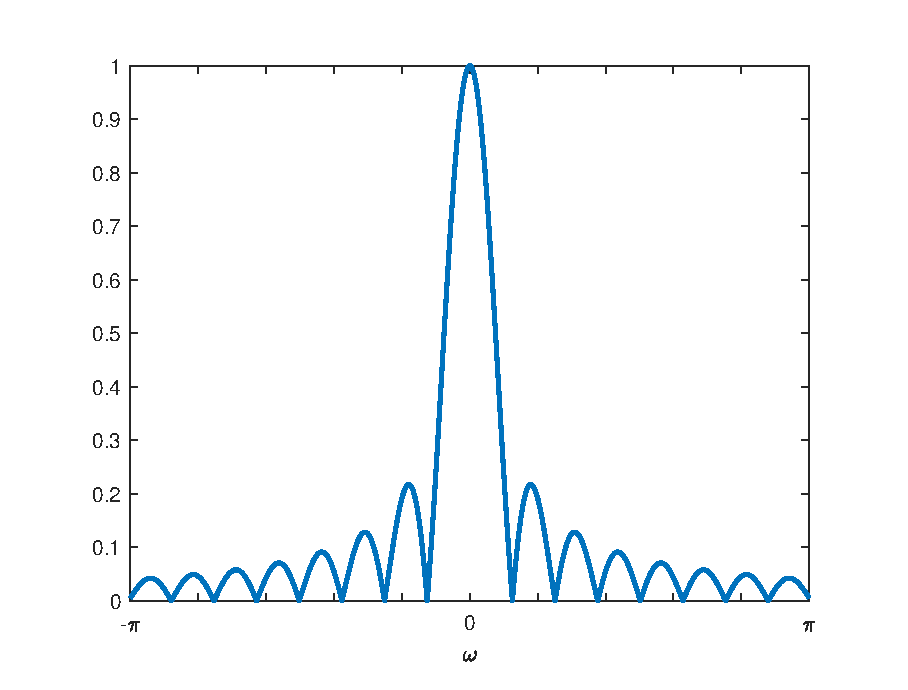
\includegraphics[width=0.6\linewidth]{sinc.eps}
    \label{sinc}
\end{figure}
在零点的时候$\omega = 0$它是多少?这明显是一啊。然后它就下来,原本它是下来的,但是我们这里取了个模,它就会开始震荡。然后怎么样?我们这里要注意,这个地方我们要强调一个事实,这个事实对于我们理解离散时间的系统很重要。因为它的这个幅度在频率轴上并不是从负无穷到正无穷。我们在上堂课就谈到过,它这个幅度啊,以$2\pi$为周期。
\begin{equation}
    H\left (  e^{j\omega} \right ) = H\left (  e^{j\left (\omega +2\pi \right )} \right ) 
\end{equation}
你看一看,我们现在这个传递函数难道不是以$2\pi$为周期吗,而且上下的符号是同时翻转的。如果是这样,这就意味着,我们去画这个频域上的事情的时候,我们应该只关注$2\pi$以内的事情。没问题吧!从$-\pi$到$\pi$,$\left [-\pi ,\pi \right ] $,是常用的选择。

通常我们就管,零附近叫低频,管正负派都叫高频。我觉得这个“高频”(High Frequency)得打一个引号,这和我们在离散时间的信号系统里那个高频不大一样。因为它究竟有多高,并不是由物理来限制,而是由采样所决定。我们待会会把这个概念更清晰地传达给大家。所以说,它这个“高”,我们要打一个引号,它并不是说物理上的高,而是接近了我们的采样频率。我们采样一旦定了,我们才有离散信号,然而离散信号一旦能够浮出水面,这意味着我们可以看到的频率最高也就是采样频率了,再高的频率我们是看不见的。好的,这是我们对于离散时间系统的一个描述。

\subsubsection{Fourier Transform}\quad

既然系统都可以这样描述了,当然我们的信号也很自然地会有使用傅里叶变换的这么一个方式来进行沟通
\begin{equation}
    \left \{ x\left (  n\right )  \right \} \longrightarrow X\left (  e^{j\omega}\right )   = \sum_{k=-\infty}^{+\infty}x(k)e^{j\omega k}
\end{equation}
这就是离散时间的傅里叶变换。
















重力是地球对物体的引力。我们常常用重力加速度来表示物体受到的引力的大小,标准重力加速度为 $9.8 \, \text{m/s}^2$。

\begin{equation}
    F = mg
\end{equation}
其中,$F$ 为重力,$m$ 为物体质量,$g$ 为重力加速度。



\newpage

% 第二章
\section{电磁学基础}

电磁学是研究电磁现象的学科,主要包括电场、磁场、电流等内容。

\subsection{库仑定律}

库仑定律描述了电荷之间的相互作用力。两个点电荷之间的相互作用力大小与电荷的乘积成正比,与它们之间的距离的平方成反比:

\begin{equation}
    F = k_e \frac{q_1 q_2}{r^2}
\end{equation}
其中,$F$ 为电荷之间的作用力,$q_1$ 和 $q_2$ 为电荷量,$r$ 为电荷之间的距离,$k_e$ 为库仑常数。

\subsection{电场}

电场是电荷间作用力的空间表现。电场强度 $\mathbf{E}$ 定义为单位电荷所受的力:

\begin{equation}
    \mathbf{E} = \frac{\mathbf{F}}{q}
\end{equation}
其中,$\mathbf{F}$ 为电场力,$q$ 为电荷量。

\newpage

% 第三章
\section{热力学}

热力学是研究热与能量转化规律的学科。热力学的基本定律包括:

\subsection{热力学第一定律}

热力学第一定律,也称能量守恒定律,表示能量既不能被创造也不能被消灭,只能从一种形式转化为另一种形式:

\begin{equation}
    \Delta U = Q - W
\end{equation}
其中,$\Delta U$ 为内能变化,$Q$ 为热量,$W$ 为功。

\subsection{热力学第二定律}

热力学第二定律表明,孤立系统的熵总是增加的,熵增原则指出自然过程趋向于无序状态。

\newpage

% 参考文献
\section{参考文献}

\begin{thebibliography}{99}
    \bibitem{ref1} 物理学原理,John D. Cutnell,Kenny W. Johnson,Wiley出版社,2018。
    \bibitem{ref2} 现代物理学导论,David J. Griffiths,Prentice Hall出版社,2005。
\end{thebibliography}

\end{document}